\documentclass[]{article}
\usepackage{lmodern}
\usepackage{amssymb,amsmath}
\usepackage{ifxetex,ifluatex}
\usepackage{fixltx2e} % provides \textsubscript
\ifnum 0\ifxetex 1\fi\ifluatex 1\fi=0 % if pdftex
  \usepackage[T1]{fontenc}
  \usepackage[utf8]{inputenc}
\else % if luatex or xelatex
  \ifxetex
    \usepackage{mathspec}
  \else
    \usepackage{fontspec}
  \fi
  \defaultfontfeatures{Ligatures=TeX,Scale=MatchLowercase}
\fi
% use upquote if available, for straight quotes in verbatim environments
\IfFileExists{upquote.sty}{\usepackage{upquote}}{}
% use microtype if available
\IfFileExists{microtype.sty}{%
\usepackage{microtype}
\UseMicrotypeSet[protrusion]{basicmath} % disable protrusion for tt fonts
}{}
\usepackage[margin=1in]{geometry}
\usepackage{hyperref}
\hypersetup{unicode=true,
            pdftitle={Exercises},
            pdfborder={0 0 0},
            breaklinks=true}
\urlstyle{same}  % don't use monospace font for urls
\usepackage{color}
\usepackage{fancyvrb}
\newcommand{\VerbBar}{|}
\newcommand{\VERB}{\Verb[commandchars=\\\{\}]}
\DefineVerbatimEnvironment{Highlighting}{Verbatim}{commandchars=\\\{\}}
% Add ',fontsize=\small' for more characters per line
\usepackage{framed}
\definecolor{shadecolor}{RGB}{248,248,248}
\newenvironment{Shaded}{\begin{snugshade}}{\end{snugshade}}
\newcommand{\AlertTok}[1]{\textcolor[rgb]{0.94,0.16,0.16}{#1}}
\newcommand{\AnnotationTok}[1]{\textcolor[rgb]{0.56,0.35,0.01}{\textbf{\textit{#1}}}}
\newcommand{\AttributeTok}[1]{\textcolor[rgb]{0.77,0.63,0.00}{#1}}
\newcommand{\BaseNTok}[1]{\textcolor[rgb]{0.00,0.00,0.81}{#1}}
\newcommand{\BuiltInTok}[1]{#1}
\newcommand{\CharTok}[1]{\textcolor[rgb]{0.31,0.60,0.02}{#1}}
\newcommand{\CommentTok}[1]{\textcolor[rgb]{0.56,0.35,0.01}{\textit{#1}}}
\newcommand{\CommentVarTok}[1]{\textcolor[rgb]{0.56,0.35,0.01}{\textbf{\textit{#1}}}}
\newcommand{\ConstantTok}[1]{\textcolor[rgb]{0.00,0.00,0.00}{#1}}
\newcommand{\ControlFlowTok}[1]{\textcolor[rgb]{0.13,0.29,0.53}{\textbf{#1}}}
\newcommand{\DataTypeTok}[1]{\textcolor[rgb]{0.13,0.29,0.53}{#1}}
\newcommand{\DecValTok}[1]{\textcolor[rgb]{0.00,0.00,0.81}{#1}}
\newcommand{\DocumentationTok}[1]{\textcolor[rgb]{0.56,0.35,0.01}{\textbf{\textit{#1}}}}
\newcommand{\ErrorTok}[1]{\textcolor[rgb]{0.64,0.00,0.00}{\textbf{#1}}}
\newcommand{\ExtensionTok}[1]{#1}
\newcommand{\FloatTok}[1]{\textcolor[rgb]{0.00,0.00,0.81}{#1}}
\newcommand{\FunctionTok}[1]{\textcolor[rgb]{0.00,0.00,0.00}{#1}}
\newcommand{\ImportTok}[1]{#1}
\newcommand{\InformationTok}[1]{\textcolor[rgb]{0.56,0.35,0.01}{\textbf{\textit{#1}}}}
\newcommand{\KeywordTok}[1]{\textcolor[rgb]{0.13,0.29,0.53}{\textbf{#1}}}
\newcommand{\NormalTok}[1]{#1}
\newcommand{\OperatorTok}[1]{\textcolor[rgb]{0.81,0.36,0.00}{\textbf{#1}}}
\newcommand{\OtherTok}[1]{\textcolor[rgb]{0.56,0.35,0.01}{#1}}
\newcommand{\PreprocessorTok}[1]{\textcolor[rgb]{0.56,0.35,0.01}{\textit{#1}}}
\newcommand{\RegionMarkerTok}[1]{#1}
\newcommand{\SpecialCharTok}[1]{\textcolor[rgb]{0.00,0.00,0.00}{#1}}
\newcommand{\SpecialStringTok}[1]{\textcolor[rgb]{0.31,0.60,0.02}{#1}}
\newcommand{\StringTok}[1]{\textcolor[rgb]{0.31,0.60,0.02}{#1}}
\newcommand{\VariableTok}[1]{\textcolor[rgb]{0.00,0.00,0.00}{#1}}
\newcommand{\VerbatimStringTok}[1]{\textcolor[rgb]{0.31,0.60,0.02}{#1}}
\newcommand{\WarningTok}[1]{\textcolor[rgb]{0.56,0.35,0.01}{\textbf{\textit{#1}}}}
\usepackage{graphicx,grffile}
\makeatletter
\def\maxwidth{\ifdim\Gin@nat@width>\linewidth\linewidth\else\Gin@nat@width\fi}
\def\maxheight{\ifdim\Gin@nat@height>\textheight\textheight\else\Gin@nat@height\fi}
\makeatother
% Scale images if necessary, so that they will not overflow the page
% margins by default, and it is still possible to overwrite the defaults
% using explicit options in \includegraphics[width, height, ...]{}
\setkeys{Gin}{width=\maxwidth,height=\maxheight,keepaspectratio}
\IfFileExists{parskip.sty}{%
\usepackage{parskip}
}{% else
\setlength{\parindent}{0pt}
\setlength{\parskip}{6pt plus 2pt minus 1pt}
}
\setlength{\emergencystretch}{3em}  % prevent overfull lines
\providecommand{\tightlist}{%
  \setlength{\itemsep}{0pt}\setlength{\parskip}{0pt}}
\setcounter{secnumdepth}{0}
% Redefines (sub)paragraphs to behave more like sections
\ifx\paragraph\undefined\else
\let\oldparagraph\paragraph
\renewcommand{\paragraph}[1]{\oldparagraph{#1}\mbox{}}
\fi
\ifx\subparagraph\undefined\else
\let\oldsubparagraph\subparagraph
\renewcommand{\subparagraph}[1]{\oldsubparagraph{#1}\mbox{}}
\fi

%%% Use protect on footnotes to avoid problems with footnotes in titles
\let\rmarkdownfootnote\footnote%
\def\footnote{\protect\rmarkdownfootnote}

%%% Change title format to be more compact
\usepackage{titling}

% Create subtitle command for use in maketitle
\providecommand{\subtitle}[1]{
  \posttitle{
    \begin{center}\large#1\end{center}
    }
}

\setlength{\droptitle}{-2em}

  \title{Exercises}
    \pretitle{\vspace{\droptitle}\centering\huge}
  \posttitle{\par}
  \subtitle{SCR week 5}
  \author{}
    \preauthor{}\postauthor{}
    \date{}
    \predate{}\postdate{}
  
\usepackage{graphicx}
\usepackage{float}
\usepackage{placeins}

\begin{document}
\maketitle

\hypertarget{exercises-part-1}{%
\section{Exercises part 1}\label{exercises-part-1}}

\hypertarget{density-plots}{%
\subsection{1.1. Density plots}\label{density-plots}}

Read paragraph 12.1.4 of the book of Norman, pp.~264 - 265. In this
exercise you will create the graph shown on page 265, but using a
different dataset, called ``tobit.csv'' (see
\texttt{0\_data/tobit.csv}). This data set contains test scores of 200
children. The variables you will use in this exercise are called
\texttt{read} and \texttt{math}.

\hypertarget{a}{%
\subsubsection{a}\label{a}}

Read in the \texttt{tobit} dataset.

\textbf{Answer:}

\begin{Shaded}
\begin{Highlighting}[]
\NormalTok{testscores <-}\StringTok{ }\KeywordTok{read.csv}\NormalTok{(}\StringTok{"0_data/tobit.csv"}\NormalTok{)}
\end{Highlighting}
\end{Shaded}

\hypertarget{b}{%
\subsubsection{b}\label{b}}

Inspect the data set by using a few \texttt{R} functions that explore
the structure of the data, or can give a summary of the data.

\textbf{Answer:}

\begin{Shaded}
\begin{Highlighting}[]
\KeywordTok{str}\NormalTok{(testscores)}
\end{Highlighting}
\end{Shaded}

\begin{verbatim}
## 'data.frame':    200 obs. of  6 variables:
##  $ X   : int  1 2 3 4 5 6 7 8 9 10 ...
##  $ id  : int  1 2 3 4 5 6 7 8 9 10 ...
##  $ read: int  34 39 63 44 47 47 57 39 48 47 ...
##  $ math: int  40 33 48 41 43 46 59 52 52 49 ...
##  $ prog: Factor w/ 3 levels "academic","general",..: 3 3 2 2 2 2 2 2 3 1 ...
##  $ apt : int  352 449 648 501 762 658 800 613 531 528 ...
\end{verbatim}

\begin{Shaded}
\begin{Highlighting}[]
\KeywordTok{summary}\NormalTok{(testscores) }\CommentTok{#inspect the data set}
\end{Highlighting}
\end{Shaded}

\begin{verbatim}
##        X                id              read            math      
##  Min.   :  1.00   Min.   :  1.00   Min.   :28.00   Min.   :33.00  
##  1st Qu.: 50.75   1st Qu.: 50.75   1st Qu.:44.00   1st Qu.:45.00  
##  Median :100.50   Median :100.50   Median :50.00   Median :52.00  
##  Mean   :100.50   Mean   :100.50   Mean   :52.23   Mean   :52.65  
##  3rd Qu.:150.25   3rd Qu.:150.25   3rd Qu.:60.00   3rd Qu.:59.00  
##  Max.   :200.00   Max.   :200.00   Max.   :76.00   Max.   :75.00  
##          prog          apt       
##  academic  : 45   Min.   :352.0  
##  general   :105   1st Qu.:575.5  
##  vocational: 50   Median :633.0  
##                   Mean   :640.0  
##                   3rd Qu.:705.2  
##                   Max.   :800.0
\end{verbatim}

\hypertarget{c}{%
\subsubsection{c}\label{c}}

Like in chapter 12.1.4 of Matloff, use \texttt{density()} to get two
seperate nonparametric density estimates of the \texttt{read} and
\texttt{math} scores. Make sure you set the \texttt{from} and
\texttt{to} arguments correctly. Use the information you got from
\textbf{b} to set these. E.g.: if scores run, say from 28 to 76, you
might want to have the density run from 20 to 84.

\textbf{Answer:}

\begin{Shaded}
\begin{Highlighting}[]
\NormalTok{d_read <-}\StringTok{ }\KeywordTok{density}\NormalTok{(testscores}\OperatorTok{$}\NormalTok{read, }\DataTypeTok{from =} \DecValTok{20}\NormalTok{, }\DataTypeTok{to =} \DecValTok{84}\NormalTok{, }\DataTypeTok{bw =} \StringTok{"SJ"}\NormalTok{)}
\NormalTok{d_math <-}\StringTok{ }\KeywordTok{density}\NormalTok{(testscores}\OperatorTok{$}\NormalTok{math, }\DataTypeTok{from =} \DecValTok{20}\NormalTok{, }\DataTypeTok{to =} \DecValTok{84}\NormalTok{, }\DataTypeTok{bw =} \StringTok{"SJ"}\NormalTok{)}
\CommentTok{# the from and to of the d_read will, in our example determine the plotting window,}
\CommentTok{# so the range for d_math can be set to the same.}
\CommentTok{# We can check with summary() or range() if all the scores fall within this range.}
\end{Highlighting}
\end{Shaded}

\hypertarget{d}{%
\subsubsection{d}\label{d}}

Put both densities into a single plot, make sure you give the different
density estimates a different colour. Any interesting differences?

\textbf{Answer:}

\begin{Shaded}
\begin{Highlighting}[]
\KeywordTok{plot}\NormalTok{(d_read, }\DataTypeTok{main =} \StringTok{""}\NormalTok{, }\DataTypeTok{xlab =} \StringTok{""}\NormalTok{)}
\KeywordTok{lines}\NormalTok{(d_math, }\DataTypeTok{col =} \StringTok{'red'}\NormalTok{)}
\end{Highlighting}
\end{Shaded}

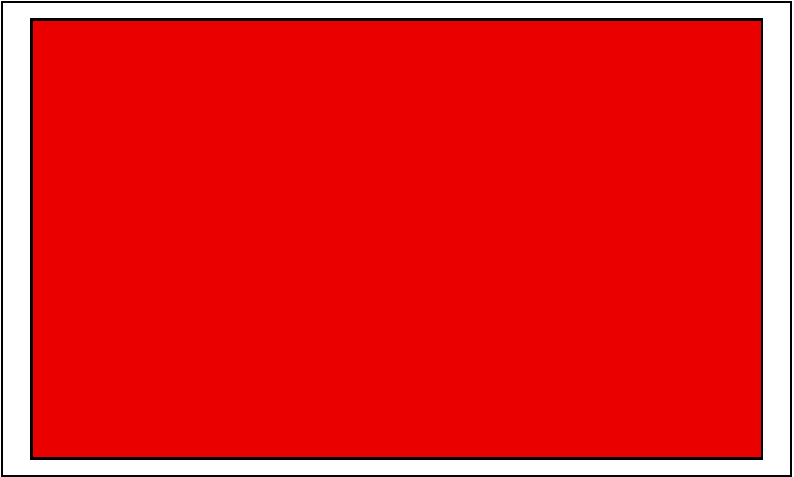
\includegraphics{w5_exercises_stats_and_visualization_answers_files/figure-latex/unnamed-chunk-4-1.pdf}
It looks as though both might be bi-modal. But that's hard to tell from
these estimates.

\hypertarget{adding-text-to-a-graph-with-help-of-the-locator-function}{%
\subsection{\texorpdfstring{1.2 Adding text to a graph with help of the
\texttt{locator()}
function}{1.2 Adding text to a graph with help of the locator() function}}\label{adding-text-to-a-graph-with-help-of-the-locator-function}}

\hypertarget{a-1}{%
\subsubsection{a}\label{a-1}}

We are going to add text to the graph created in the previous exercise.
Read par. 12.1.8 and 12.1.9 of the book of Matloff, pp.~270 - 271.
Instead of the text ``Exam 1'' and ``Exam 2'', we use now \texttt{read}
and \texttt{math} from the \texttt{tobit} data used in the previous
exercise. To determine the coordinates of the text, use the function
\texttt{locator()}. In your console, type \texttt{locator(2)} and use
enter. Then, go to the graph you created in Exercise 2 and click on the
two points in the graph where you want to put the text. Use these
coordinates in the function \texttt{text()}.

\textbf{Answer:}

\begin{Shaded}
\begin{Highlighting}[]
\CommentTok{#locator(2)}
\KeywordTok{plot}\NormalTok{(d_read, }\DataTypeTok{main =} \StringTok{""}\NormalTok{, }\DataTypeTok{xlab =} \StringTok{""}\NormalTok{)}
\KeywordTok{lines}\NormalTok{(d_math, }\DataTypeTok{col =} \StringTok{'red'}\NormalTok{)}
\KeywordTok{text}\NormalTok{(}\FloatTok{40.5}\NormalTok{,  }\FloatTok{0.038}\NormalTok{, }\StringTok{"read"}\NormalTok{)}
\KeywordTok{text}\NormalTok{(}\FloatTok{61.9}\NormalTok{, }\FloatTok{0.034}\NormalTok{, }\StringTok{"math"}\NormalTok{)}
\end{Highlighting}
\end{Shaded}

\includegraphics{w5_exercises_stats_and_visualization_answers_files/figure-latex/unnamed-chunk-5-1.pdf}

\hypertarget{b-1}{%
\subsubsection{b}\label{b-1}}

Change the size of the text by varying the \texttt{cex} parameter (See
also par. 12.2.1 on p.~272 of the book of Matloff).

\textbf{Answer:}

\begin{Shaded}
\begin{Highlighting}[]
\KeywordTok{plot}\NormalTok{(d_read, }\DataTypeTok{main =} \StringTok{""}\NormalTok{, }\DataTypeTok{xlab =} \StringTok{""}\NormalTok{)}
\KeywordTok{lines}\NormalTok{(d_math, }\DataTypeTok{col =} \StringTok{'red'}\NormalTok{)}
\KeywordTok{text}\NormalTok{(}\FloatTok{40.5}\NormalTok{,  }\FloatTok{0.038}\NormalTok{, }\StringTok{"read"}\NormalTok{, }\DataTypeTok{cex =} \FloatTok{0.6}\NormalTok{)}
\KeywordTok{text}\NormalTok{(}\FloatTok{61.9}\NormalTok{, }\FloatTok{0.034}\NormalTok{, }\StringTok{"math"}\NormalTok{, }\DataTypeTok{cex =} \FloatTok{0.6}\NormalTok{)}
\end{Highlighting}
\end{Shaded}

\includegraphics{w5_exercises_stats_and_visualization_answers_files/figure-latex/unnamed-chunk-6-1.pdf}

\hypertarget{c-1}{%
\subsubsection{c}\label{c-1}}

Add a legend to the plot using \texttt{legend()}. Put it in the topright
corner of the plot.

\textbf{Answer:}

\begin{Shaded}
\begin{Highlighting}[]
\KeywordTok{plot}\NormalTok{(d_read, }\DataTypeTok{main =} \StringTok{""}\NormalTok{, }\DataTypeTok{xlab =} \StringTok{""}\NormalTok{)}
\KeywordTok{lines}\NormalTok{(d_math, }\DataTypeTok{col =} \StringTok{'red'}\NormalTok{)}
\KeywordTok{text}\NormalTok{(}\FloatTok{40.5}\NormalTok{,  }\FloatTok{0.038}\NormalTok{, }\StringTok{"read"}\NormalTok{, }\DataTypeTok{cex =} \FloatTok{0.6}\NormalTok{)}
\KeywordTok{text}\NormalTok{(}\FloatTok{61.9}\NormalTok{, }\FloatTok{0.034}\NormalTok{, }\StringTok{"math"}\NormalTok{, }\DataTypeTok{cex =} \FloatTok{0.6}\NormalTok{)}
\KeywordTok{legend}\NormalTok{(}\DataTypeTok{x =} \StringTok{"topright"}\NormalTok{, }
       \DataTypeTok{legend =} \KeywordTok{c}\NormalTok{(}\StringTok{"dens read"}\NormalTok{, }\StringTok{"dens math"}\NormalTok{), }
       \DataTypeTok{lty =} \DecValTok{1}\NormalTok{, }\DataTypeTok{col =}  \KeywordTok{c}\NormalTok{(}\StringTok{'black'}\NormalTok{, }\StringTok{'red'}\NormalTok{)}
\NormalTok{)}
\end{Highlighting}
\end{Shaded}

\includegraphics{w5_exercises_stats_and_visualization_answers_files/figure-latex/unnamed-chunk-7-1.pdf}

\hypertarget{adding-points-to-a-graph-and-customizing-a-graph}{%
\subsection{1.3 Adding points to a graph and customizing a
graph}\label{adding-points-to-a-graph-and-customizing-a-graph}}

Let's start from scratch!

\hypertarget{a-2}{%
\subsubsection{a}\label{a-2}}

We are going to add points to an existing, but empty, graph with the
function \texttt{points()}. Look at the following code. Take special
care to try to see what the second line does. Play around with some of
the arguments if you're not sure what's going on.

\begin{Shaded}
\begin{Highlighting}[]
\KeywordTok{set.seed}\NormalTok{(}\DecValTok{99}\NormalTok{)}
\KeywordTok{plot}\NormalTok{(}\OperatorTok{-}\DecValTok{4}\OperatorTok{:}\DecValTok{4}\NormalTok{, }\DecValTok{-4}\OperatorTok{:}\DecValTok{4}\NormalTok{, }\DataTypeTok{type =} \StringTok{"n"}\NormalTok{)  }\CommentTok{# setting up coord. system}
\KeywordTok{points}\NormalTok{(}\KeywordTok{rnorm}\NormalTok{(}\DecValTok{200}\NormalTok{), }\KeywordTok{rnorm}\NormalTok{(}\DecValTok{200}\NormalTok{), }\DataTypeTok{col =} \StringTok{"red"}\NormalTok{)}
\KeywordTok{points}\NormalTok{(}\KeywordTok{rnorm}\NormalTok{(}\DecValTok{100}\NormalTok{)}\OperatorTok{/}\DecValTok{2}\NormalTok{, }\KeywordTok{rnorm}\NormalTok{(}\DecValTok{100}\NormalTok{)}\OperatorTok{/}\DecValTok{2}\NormalTok{, }\DataTypeTok{col =} \StringTok{"blue"}\NormalTok{, }\DataTypeTok{cex =} \FloatTok{1.5}\NormalTok{)}
\end{Highlighting}
\end{Shaded}

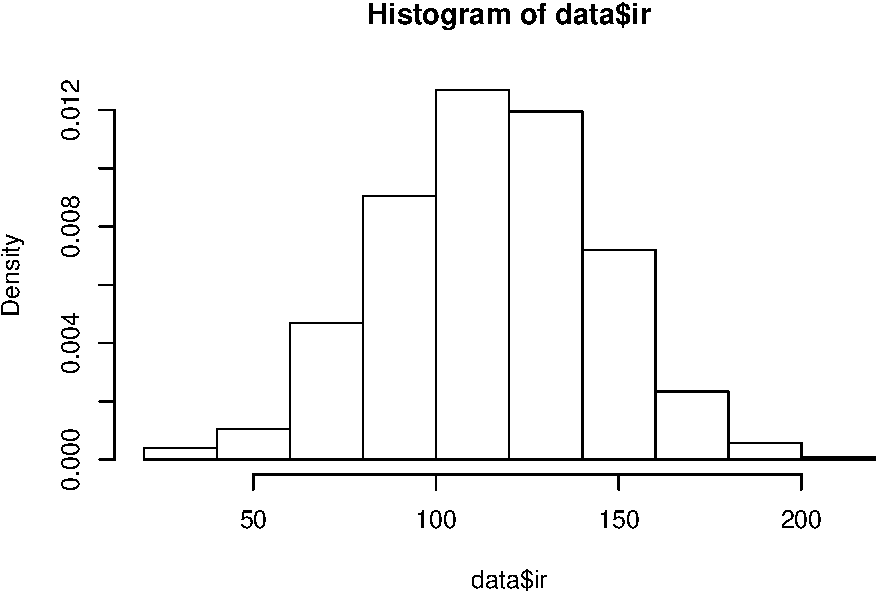
\includegraphics{w5_exercises_stats_and_visualization_answers_files/figure-latex/unnamed-chunk-8-1.pdf}

\textbf{Answer:}

The second line plots 4 points, but we told \texttt{R} to \texttt{n}ot
show them (see the \texttt{type} argument).

\hypertarget{b-2}{%
\subsubsection{b}\label{b-2}}

Change the symbol of the points used in the graph created in \textbf{a},
to a \texttt{+}, by adapting the parameter \texttt{pch} (see e.g.~the
helpfile of \texttt{points}).

\textbf{Answer:}

\begin{Shaded}
\begin{Highlighting}[]
\KeywordTok{plot}\NormalTok{(}\OperatorTok{-}\DecValTok{4}\OperatorTok{:}\DecValTok{4}\NormalTok{, }\DecValTok{-4}\OperatorTok{:}\DecValTok{4}\NormalTok{, }\DataTypeTok{type =} \StringTok{"n"}\NormalTok{)  }\CommentTok{# setting up coord. system}
\KeywordTok{points}\NormalTok{(}\KeywordTok{rnorm}\NormalTok{(}\DecValTok{200}\NormalTok{), }\KeywordTok{rnorm}\NormalTok{(}\DecValTok{200}\NormalTok{), }\DataTypeTok{pch =} \StringTok{"+"}\NormalTok{, }\DataTypeTok{col =} \StringTok{"red"}\NormalTok{)}
\KeywordTok{points}\NormalTok{(}\KeywordTok{rnorm}\NormalTok{(}\DecValTok{100}\NormalTok{)}\OperatorTok{/}\DecValTok{2}\NormalTok{, }\KeywordTok{rnorm}\NormalTok{(}\DecValTok{100}\NormalTok{)}\OperatorTok{/}\DecValTok{2}\NormalTok{, }\DataTypeTok{pch =} \StringTok{"+"}\NormalTok{, }\DataTypeTok{col =} \StringTok{"blue"}\NormalTok{)}
\end{Highlighting}
\end{Shaded}

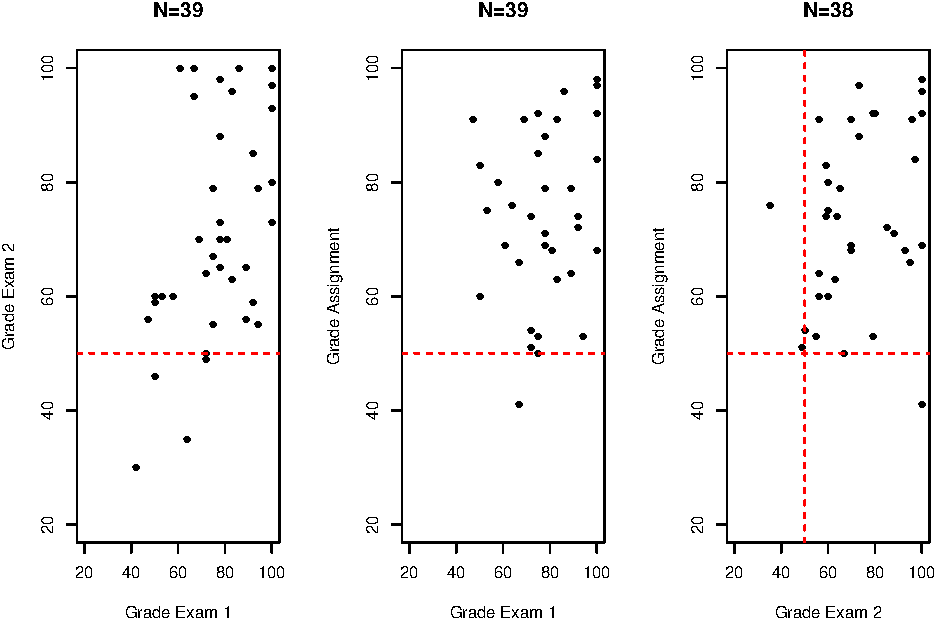
\includegraphics{w5_exercises_stats_and_visualization_answers_files/figure-latex/unnamed-chunk-9-1.pdf}

\hypertarget{c-2}{%
\subsubsection{c}\label{c-2}}

Change the color of the points, by adapting the parameter \texttt{col}.
Use \texttt{colors()} to inspect which colors are available in
\texttt{R}. Go nuts with colours by using e.g. \texttt{rainbow()}.

\textbf{Answer:}

\begin{Shaded}
\begin{Highlighting}[]
\KeywordTok{plot}\NormalTok{(}\OperatorTok{-}\DecValTok{4}\OperatorTok{:}\DecValTok{4}\NormalTok{, }\DecValTok{-4}\OperatorTok{:}\DecValTok{4}\NormalTok{, }\DataTypeTok{type =} \StringTok{"n"}\NormalTok{)  }\CommentTok{# setting up coord. system}
\KeywordTok{points}\NormalTok{(}\KeywordTok{rnorm}\NormalTok{(}\DecValTok{200}\NormalTok{), }\KeywordTok{rnorm}\NormalTok{(}\DecValTok{200}\NormalTok{), }\DataTypeTok{pch =} \DecValTok{19}\NormalTok{, }\DataTypeTok{col =} \StringTok{"darkgreen"}\NormalTok{)}
\KeywordTok{points}\NormalTok{(}\KeywordTok{rnorm}\NormalTok{(}\DecValTok{100}\NormalTok{)}\OperatorTok{/}\DecValTok{2}\NormalTok{, }\KeywordTok{rnorm}\NormalTok{(}\DecValTok{100}\NormalTok{)}\OperatorTok{/}\DecValTok{2}\NormalTok{, }\DataTypeTok{pch =} \DecValTok{19}\NormalTok{, }\DataTypeTok{col =} \StringTok{"wheat2"}\NormalTok{)}
\end{Highlighting}
\end{Shaded}

\includegraphics{w5_exercises_stats_and_visualization_answers_files/figure-latex/unnamed-chunk-10-1.pdf}

\hypertarget{d-1}{%
\subsubsection{d}\label{d-1}}

Change the range of the x-axis and y-axis (using \texttt{xlim} and
\texttt{ylim}; see also paragraph 12.2.2, p.~273 of Matloff).

\textbf{Answer:}

\begin{Shaded}
\begin{Highlighting}[]
\CommentTok{# the following three lines all work towards the same end,}
\CommentTok{# although in slightly different ways, all are correct.}
\KeywordTok{plot}\NormalTok{(}\OperatorTok{-}\DecValTok{4}\OperatorTok{:}\DecValTok{4}\NormalTok{, }\DecValTok{-4}\OperatorTok{:}\DecValTok{4}\NormalTok{, }\DataTypeTok{type =} \StringTok{'n'}\NormalTok{, }\DataTypeTok{xlim =} \KeywordTok{c}\NormalTok{(}\OperatorTok{-}\DecValTok{8}\NormalTok{, }\DecValTok{8}\NormalTok{), }\DataTypeTok{ylim =} \KeywordTok{c}\NormalTok{(}\OperatorTok{-}\DecValTok{8}\NormalTok{, }\DecValTok{8}\NormalTok{))}
\end{Highlighting}
\end{Shaded}

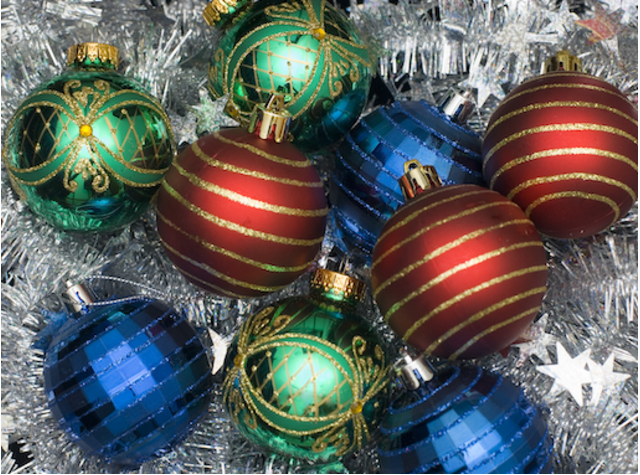
\includegraphics{w5_exercises_stats_and_visualization_answers_files/figure-latex/unnamed-chunk-11-1.pdf}

\begin{Shaded}
\begin{Highlighting}[]
\KeywordTok{plot}\NormalTok{(}\OperatorTok{-}\DecValTok{8}\OperatorTok{:}\DecValTok{8}\NormalTok{, }\DecValTok{-8}\OperatorTok{:}\DecValTok{8}\NormalTok{, }\DataTypeTok{type =} \StringTok{'n'}\NormalTok{)}
\end{Highlighting}
\end{Shaded}

\includegraphics{w5_exercises_stats_and_visualization_answers_files/figure-latex/unnamed-chunk-11-2.pdf}

\begin{Shaded}
\begin{Highlighting}[]
\KeywordTok{plot}\NormalTok{(}\OtherTok{NULL}\NormalTok{,  }\DataTypeTok{xlim =} \KeywordTok{c}\NormalTok{(}\OperatorTok{-}\DecValTok{8}\NormalTok{, }\DecValTok{8}\NormalTok{),  }\DataTypeTok{ylim =} \KeywordTok{c}\NormalTok{(}\OperatorTok{-}\DecValTok{8}\NormalTok{, }\DecValTok{8}\NormalTok{))}
\KeywordTok{points}\NormalTok{(}\KeywordTok{rnorm}\NormalTok{(}\DecValTok{200}\NormalTok{), }\KeywordTok{rnorm}\NormalTok{(}\DecValTok{200}\NormalTok{), }\DataTypeTok{pch =} \DecValTok{19}\NormalTok{, }\DataTypeTok{col =} \StringTok{"darkgreen"}\NormalTok{) }
\KeywordTok{points}\NormalTok{(}\KeywordTok{rnorm}\NormalTok{(}\DecValTok{100}\NormalTok{)}\OperatorTok{/}\DecValTok{2}\NormalTok{, }\KeywordTok{rnorm}\NormalTok{(}\DecValTok{100}\NormalTok{)}\OperatorTok{/}\DecValTok{2}\NormalTok{, }\DataTypeTok{pch =} \DecValTok{19}\NormalTok{, }\DataTypeTok{col =} \StringTok{"wheat2"}\NormalTok{)}
\end{Highlighting}
\end{Shaded}

\includegraphics{w5_exercises_stats_and_visualization_answers_files/figure-latex/unnamed-chunk-11-3.pdf}

\hypertarget{e}{%
\subsubsection{e}\label{e}}

Change the labels of the x-axis and y-axis (using \texttt{xlab} and
\texttt{ylab}) and create a title above the plot (using \texttt{main}).

\textbf{Answer:}

\begin{Shaded}
\begin{Highlighting}[]
\KeywordTok{plot}\NormalTok{(}\OtherTok{NULL}\NormalTok{,  }\DataTypeTok{xlim =} \KeywordTok{c}\NormalTok{(}\OperatorTok{-}\DecValTok{8}\NormalTok{, }\DecValTok{8}\NormalTok{),  }\DataTypeTok{ylim =} \KeywordTok{c}\NormalTok{(}\OperatorTok{-}\DecValTok{8}\NormalTok{, }\DecValTok{8}\NormalTok{), }\DataTypeTok{xlab =} \StringTok{"variable X1"}\NormalTok{, }\DataTypeTok{ylab =} \StringTok{"variable X2"}\NormalTok{)  }
\KeywordTok{points}\NormalTok{(}\KeywordTok{rnorm}\NormalTok{(}\DecValTok{200}\NormalTok{), }\KeywordTok{rnorm}\NormalTok{(}\DecValTok{200}\NormalTok{), }\DataTypeTok{pch =} \DecValTok{19}\NormalTok{, }\DataTypeTok{col =} \StringTok{"darkgreen"}\NormalTok{)}
\KeywordTok{points}\NormalTok{(}\KeywordTok{rnorm}\NormalTok{(}\DecValTok{100}\NormalTok{)}\OperatorTok{/}\DecValTok{2}\NormalTok{, }\KeywordTok{rnorm}\NormalTok{(}\DecValTok{100}\NormalTok{)}\OperatorTok{/}\DecValTok{2}\NormalTok{, }\DataTypeTok{pch =} \DecValTok{19}\NormalTok{, }\DataTypeTok{col =} \StringTok{"wheat2"}\NormalTok{)}
\end{Highlighting}
\end{Shaded}

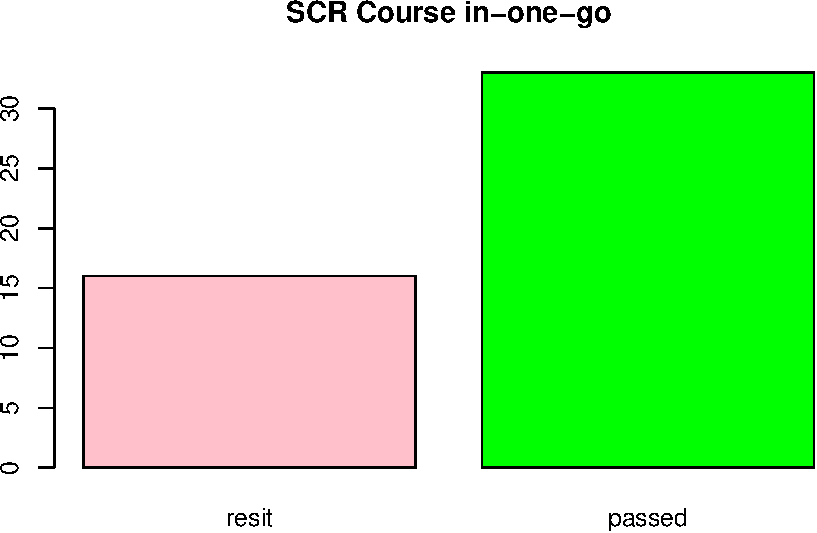
\includegraphics{w5_exercises_stats_and_visualization_answers_files/figure-latex/unnamed-chunk-12-1.pdf}

\hypertarget{plotting-the-chi-square-density-function}{%
\subsection{1.4 Plotting the chi-square density
function}\label{plotting-the-chi-square-density-function}}

\hypertarget{a-3}{%
\subsubsection{a}\label{a-3}}

Create a graph of the chi-square density function with \(df = 10\) (df =
degrees of freedom). Make sure that you set the limits of your y-axis to
0 and 0.30 and the limits of the x-axis to 0 and 32.5.

\textbf{Answer:}

\begin{Shaded}
\begin{Highlighting}[]
\NormalTok{x_ax <-}\StringTok{ }\KeywordTok{seq}\NormalTok{(}\DecValTok{0}\NormalTok{, }\FloatTok{32.5}\NormalTok{, }\DataTypeTok{length =} \DecValTok{1000}\NormalTok{)}
\KeywordTok{plot}\NormalTok{(x_ax, }\KeywordTok{dchisq}\NormalTok{(x_ax, }\DataTypeTok{df =} \DecValTok{10}\NormalTok{), }
  \DataTypeTok{type =} \StringTok{"l"}\NormalTok{, }\DataTypeTok{xlab =} \StringTok{"x value"}\NormalTok{, }\DataTypeTok{ylab =} \StringTok{"Density"}\NormalTok{, }
  \DataTypeTok{ylim =} \KeywordTok{c}\NormalTok{(}\DecValTok{0}\NormalTok{, }\FloatTok{0.30}\NormalTok{), }\DataTypeTok{xlim =} \KeywordTok{c}\NormalTok{(}\DecValTok{0}\NormalTok{, }\FloatTok{32.5}\NormalTok{), }
  \DataTypeTok{main =} \StringTok{"chi-square distribution"}
\NormalTok{)}
\end{Highlighting}
\end{Shaded}

\includegraphics{w5_exercises_stats_and_visualization_answers_files/figure-latex/unnamed-chunk-13-1.pdf}

\hypertarget{b-3}{%
\subsubsection{b}\label{b-3}}

Use the function \texttt{lines()} to add more chi-square distributions,
differing in number of degrees of freedom, to the graph created in a.
Use \(df = 1\), \(df = 3\) and \(df = 5\). Add a suitable legend to the
graph. Think about the limits we made you set in \textbf{a}, why do you
think we suggested these limits?

\textbf{Answer:}

\begin{Shaded}
\begin{Highlighting}[]
\KeywordTok{plot}\NormalTok{(}\OtherTok{NULL}\NormalTok{, }\DataTypeTok{type =} \StringTok{"l"}\NormalTok{, }
  \DataTypeTok{xlab =} \StringTok{"x value"}\NormalTok{, }\DataTypeTok{ylab =} \StringTok{"Density"}\NormalTok{, }
  \DataTypeTok{ylim =} \KeywordTok{c}\NormalTok{(}\DecValTok{0}\NormalTok{, }\FloatTok{0.30}\NormalTok{), }\DataTypeTok{xlim =} \KeywordTok{c}\NormalTok{(}\DecValTok{0}\NormalTok{, }\FloatTok{32.5}\NormalTok{), }
  \DataTypeTok{main =} \StringTok{"chi-square distribution"}
\NormalTok{)}
\NormalTok{degf <-}\StringTok{ }\KeywordTok{c}\NormalTok{(}\DecValTok{1}\NormalTok{, }\DecValTok{3}\NormalTok{, }\DecValTok{5}\NormalTok{, }\DecValTok{10}\NormalTok{)}
\NormalTok{colors <-}\StringTok{ }\KeywordTok{c}\NormalTok{(}\StringTok{"red"}\NormalTok{, }\StringTok{"blue"}\NormalTok{, }\StringTok{"darkgreen"}\NormalTok{, }\StringTok{"black"}\NormalTok{)}
\NormalTok{labels <-}\StringTok{ }\KeywordTok{c}\NormalTok{(}\StringTok{"df = 1"}\NormalTok{, }\StringTok{"df = 3"}\NormalTok{, }\StringTok{"df = 5"}\NormalTok{, }\StringTok{"df = 10"}\NormalTok{)}
\ControlFlowTok{for}\NormalTok{ (i }\ControlFlowTok{in} \DecValTok{1}\OperatorTok{:}\KeywordTok{length}\NormalTok{(degf)) \{}
  \KeywordTok{lines}\NormalTok{(x_ax, }\KeywordTok{dchisq}\NormalTok{(x_ax, degf[i]), }\DataTypeTok{col =}\NormalTok{ colors[i])}
\NormalTok{\}}
\KeywordTok{legend}\NormalTok{(}\StringTok{"topright"}\NormalTok{, }\DataTypeTok{inset =} \FloatTok{.05}\NormalTok{, labels, }\DataTypeTok{lty =} \KeywordTok{rep}\NormalTok{(}\DecValTok{1}\NormalTok{, }\DecValTok{4}\NormalTok{), }\DataTypeTok{col =}\NormalTok{ colors)}
\end{Highlighting}
\end{Shaded}

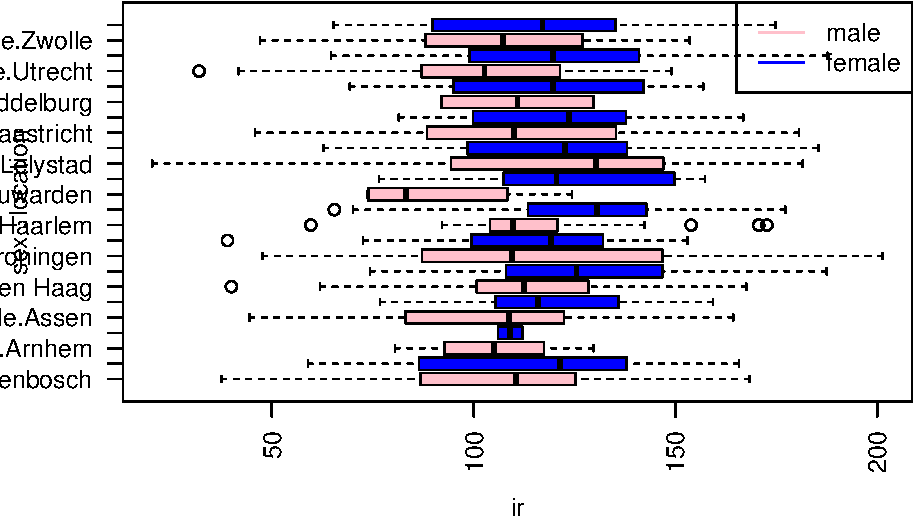
\includegraphics{w5_exercises_stats_and_visualization_answers_files/figure-latex/unnamed-chunk-14-1.pdf}

We suggested those limits, as the default limits of the first plot would
mean some of the lines would be outside of the plotting window.

\hypertarget{c-3}{%
\subsubsection{c}\label{c-3}}

Look at the helpfile of the function \texttt{curve}. See if you can
produce the plot in the previous exercise, using the \texttt{curve}
function.

\textbf{Answer:}

\begin{Shaded}
\begin{Highlighting}[]
\CommentTok{#solution to a}
\KeywordTok{plot}\NormalTok{(}\OtherTok{NULL}\NormalTok{, }\DataTypeTok{type =} \StringTok{"l"}\NormalTok{, }
  \DataTypeTok{xlab =} \StringTok{"x value"}\NormalTok{, }\DataTypeTok{ylab =} \StringTok{"Density"}\NormalTok{, }
  \DataTypeTok{ylim =} \KeywordTok{c}\NormalTok{(}\DecValTok{0}\NormalTok{, }\FloatTok{0.30}\NormalTok{), }\DataTypeTok{xlim =} \KeywordTok{c}\NormalTok{(}\DecValTok{0}\NormalTok{, }\FloatTok{32.5}\NormalTok{), }
  \DataTypeTok{main =} \StringTok{"chi-square distribution"}
\NormalTok{)}
\CommentTok{#solution to b}
\NormalTok{degf <-}\StringTok{ }\KeywordTok{c}\NormalTok{(}\DecValTok{1}\NormalTok{, }\DecValTok{3}\NormalTok{, }\DecValTok{5}\NormalTok{, }\DecValTok{10}\NormalTok{)}
\NormalTok{colors <-}\StringTok{ }\KeywordTok{c}\NormalTok{(}\StringTok{"red"}\NormalTok{, }\StringTok{"blue"}\NormalTok{, }\StringTok{"darkgreen"}\NormalTok{, }\StringTok{"black"}\NormalTok{)}
\NormalTok{labels <-}\StringTok{ }\KeywordTok{c}\NormalTok{(}\StringTok{"df = 1"}\NormalTok{, }\StringTok{"df = 3"}\NormalTok{, }\StringTok{"df = 5"}\NormalTok{, }\StringTok{"df = 10"}\NormalTok{)}

\CommentTok{# this is where the answer differs:}
\NormalTok{mydchisq <-}\StringTok{ }\ControlFlowTok{function}\NormalTok{(x, df) \{}
  \KeywordTok{return}\NormalTok{(}\KeywordTok{dchisq}\NormalTok{(x, df))}
\NormalTok{\}}
\ControlFlowTok{for}\NormalTok{ (i }\ControlFlowTok{in} \DecValTok{1}\OperatorTok{:}\KeywordTok{length}\NormalTok{(degf)) \{}
  \KeywordTok{curve}\NormalTok{(}\KeywordTok{mydchisq}\NormalTok{(x, degf[i]), }\DataTypeTok{col =}\NormalTok{ colors[i], }\DataTypeTok{add =} \OtherTok{TRUE}\NormalTok{, }\DataTypeTok{n =} \DecValTok{1000}\NormalTok{)}
\NormalTok{\}}
\KeywordTok{legend}\NormalTok{(}\StringTok{"topright"}\NormalTok{, }\DataTypeTok{inset =} \FloatTok{.05}\NormalTok{, labels, }\DataTypeTok{lty =} \KeywordTok{rep}\NormalTok{(}\DecValTok{1}\NormalTok{, }\DecValTok{4}\NormalTok{), }\DataTypeTok{col =}\NormalTok{ colors)}
\end{Highlighting}
\end{Shaded}

\includegraphics{w5_exercises_stats_and_visualization_answers_files/figure-latex/unnamed-chunk-15-1.pdf}

\hypertarget{d-2}{%
\subsubsection{d}\label{d-2}}

Sample a 1000 random values from a chisquare distribution with degrees
of freedom equal to 3. Plot the results using a histogram. Use the code
you've written in \textbf{b} (and/or \textbf{c}) to add the theoritical
density lines to the histogram. Which theoretical density best matches
the empirical distribution given by the histogram?

\textbf{Answer:}

\begin{Shaded}
\begin{Highlighting}[]
\NormalTok{my_chisq_sample <-}\StringTok{ }\KeywordTok{rchisq}\NormalTok{(}\DecValTok{1000}\NormalTok{, }\DataTypeTok{df =} \DecValTok{5}\NormalTok{)}

\KeywordTok{hist}\NormalTok{(my_chisq_sample, }\DataTypeTok{breaks =} \StringTok{"fd"}\NormalTok{, }\DataTypeTok{freq =} \OtherTok{FALSE}\NormalTok{, }\DataTypeTok{col =} \StringTok{'lightyellow'}\NormalTok{)}
\NormalTok{degf <-}\StringTok{ }\KeywordTok{c}\NormalTok{(}\DecValTok{1}\NormalTok{, }\DecValTok{3}\NormalTok{, }\DecValTok{5}\NormalTok{, }\DecValTok{10}\NormalTok{)}
\NormalTok{colors <-}\StringTok{ }\KeywordTok{c}\NormalTok{(}\StringTok{"red"}\NormalTok{, }\StringTok{"blue"}\NormalTok{, }\StringTok{"darkgreen"}\NormalTok{, }\StringTok{"black"}\NormalTok{)}
\NormalTok{labels <-}\StringTok{ }\KeywordTok{c}\NormalTok{(}\StringTok{"df = 1"}\NormalTok{, }\StringTok{"df = 3"}\NormalTok{, }\StringTok{"df = 5"}\NormalTok{, }\StringTok{"df = 10"}\NormalTok{)}

\ControlFlowTok{for}\NormalTok{ (i }\ControlFlowTok{in} \DecValTok{1}\OperatorTok{:}\KeywordTok{length}\NormalTok{(degf)) \{}
  \KeywordTok{curve}\NormalTok{(}\KeywordTok{mydchisq}\NormalTok{(x, degf[i]), }\DataTypeTok{col =}\NormalTok{ colors[i], }\DataTypeTok{add =} \OtherTok{TRUE}\NormalTok{, }\DataTypeTok{n =} \DecValTok{1000}\NormalTok{, }\DataTypeTok{lwd =} \DecValTok{2}\NormalTok{)}
\NormalTok{\}}
\KeywordTok{legend}\NormalTok{(}\StringTok{"topright"}\NormalTok{, }\DataTypeTok{inset =} \FloatTok{.05}\NormalTok{, labels, }\DataTypeTok{lty =} \KeywordTok{rep}\NormalTok{(}\DecValTok{1}\NormalTok{, }\DecValTok{4}\NormalTok{), }\DataTypeTok{col =}\NormalTok{ colors, }\DataTypeTok{lwd =} \DecValTok{2}\NormalTok{)}
\end{Highlighting}
\end{Shaded}

\includegraphics{w5_exercises_stats_and_visualization_answers_files/figure-latex/unnamed-chunk-16-1.pdf}

\hypertarget{plotting-some-categorical-data}{%
\subsection{1.5 Plotting some categorical
data}\label{plotting-some-categorical-data}}

Suppose we have the following variable:

\begin{Shaded}
\begin{Highlighting}[]
\NormalTok{observed_haircolours <-}\StringTok{ }\KeywordTok{c}\NormalTok{(}\StringTok{"blonde"}\NormalTok{ =}\StringTok{  }\DecValTok{10}\NormalTok{, }\StringTok{"brown"}\NormalTok{ =}\StringTok{ }\DecValTok{14}\NormalTok{, }\StringTok{"black"}\NormalTok{ =}\StringTok{ }\DecValTok{3}\NormalTok{, }\StringTok{"red"}\NormalTok{ =}\StringTok{ }\DecValTok{2}\NormalTok{)}
\end{Highlighting}
\end{Shaded}

where each entry represents the number of times the specified
haircolours were observed in a sample of 29 people.

\hypertarget{a-4}{%
\subsubsection{a}\label{a-4}}

Use \texttt{plot} to plot the observed haircolours. Is this plot any
good?

\textbf{Answer:}

\begin{Shaded}
\begin{Highlighting}[]
\KeywordTok{plot}\NormalTok{(observed_haircolours)}
\end{Highlighting}
\end{Shaded}

\includegraphics{w5_exercises_stats_and_visualization_answers_files/figure-latex/unnamed-chunk-18-1.pdf}
This isn't very useful.

\hypertarget{b-4}{%
\subsubsection{b}\label{b-4}}

Now use \texttt{barplot} and \texttt{pie}. Are these any better?

\textbf{Answer:}

\begin{Shaded}
\begin{Highlighting}[]
\KeywordTok{barplot}\NormalTok{(observed_haircolours)}
\end{Highlighting}
\end{Shaded}

\includegraphics{w5_exercises_stats_and_visualization_answers_files/figure-latex/unnamed-chunk-19-1.pdf}

\begin{Shaded}
\begin{Highlighting}[]
\KeywordTok{pie}\NormalTok{(observed_haircolours)}
\end{Highlighting}
\end{Shaded}

\includegraphics{w5_exercises_stats_and_visualization_answers_files/figure-latex/unnamed-chunk-19-2.pdf}
Yes much better, these are graphs that tell us something interesting.

\hypertarget{c-4}{%
\subsubsection{c}\label{c-4}}

Convert the variable \texttt{observed\_haircolours} to a table (recall
e.g.~the \texttt{as.numeric} function).

\textbf{Answer:}

\begin{Shaded}
\begin{Highlighting}[]
\NormalTok{oh_table <-}\StringTok{ }\KeywordTok{as.table}\NormalTok{(observed_haircolours)}
\end{Highlighting}
\end{Shaded}

\hypertarget{d-3}{%
\subsubsection{d}\label{d-3}}

Use \texttt{plot} on this object. What do you think of this plot?

\textbf{Answer:}

\begin{Shaded}
\begin{Highlighting}[]
\KeywordTok{plot}\NormalTok{(oh_table)}
\end{Highlighting}
\end{Shaded}

\includegraphics{w5_exercises_stats_and_visualization_answers_files/figure-latex/unnamed-chunk-21-1.pdf}
better than \texttt{plot} of the original, but still not very nice.

\hypertarget{e-1}{%
\subsubsection{e}\label{e-1}}

Use \texttt{barplot} and \texttt{pie} again, this time on your variable
that's a table. Are they different from the ones you made in \textbf{b}?

\textbf{Answer:}

\begin{Shaded}
\begin{Highlighting}[]
\KeywordTok{barplot}\NormalTok{(oh_table)}
\end{Highlighting}
\end{Shaded}

\includegraphics{w5_exercises_stats_and_visualization_answers_files/figure-latex/unnamed-chunk-22-1.pdf}

\begin{Shaded}
\begin{Highlighting}[]
\KeywordTok{pie}\NormalTok{(oh_table)}
\end{Highlighting}
\end{Shaded}

\includegraphics{w5_exercises_stats_and_visualization_answers_files/figure-latex/unnamed-chunk-22-2.pdf}
No, not different.

\hypertarget{f}{%
\subsubsection{f}\label{f}}

Turn the variable \texttt{observed\_haircolours} into a factor. Make a
plot of this new variable. What type of plot is it? Do you think this
plot has anything interesting to say?

\textbf{Answer:}

\begin{Shaded}
\begin{Highlighting}[]
\KeywordTok{plot}\NormalTok{(}\KeywordTok{factor}\NormalTok{(observed_haircolours))}
\end{Highlighting}
\end{Shaded}

\includegraphics{w5_exercises_stats_and_visualization_answers_files/figure-latex/unnamed-chunk-23-1.pdf}
It's a barplot. The plot itself is not interesting at all. It just takes
the values \texttt{2}, \texttt{3}, \texttt{10} and \texttt{14}, and acts
as if each has been observed a single time.

\hypertarget{g}{%
\subsubsection{g}\label{g}}

Use \texttt{rep} to create a \texttt{factor} variable that contains the
entries \texttt{blonde}, \texttt{brown}, \texttt{black} and
\texttt{red}, as many times as given in \texttt{observed\_haircolours}.

\textbf{Answer:}

\begin{Shaded}
\begin{Highlighting}[]
\NormalTok{oh_factor <-}\StringTok{ }\KeywordTok{factor}\NormalTok{(}\KeywordTok{rep}\NormalTok{(}\KeywordTok{names}\NormalTok{(observed_haircolours), observed_haircolours))}
\end{Highlighting}
\end{Shaded}

\hypertarget{h}{%
\subsubsection{h}\label{h}}

Use \texttt{plot} on this \texttt{factor}. Is this any better than in
\textbf{f}?

\textbf{Answer:}

\begin{Shaded}
\begin{Highlighting}[]
\KeywordTok{plot}\NormalTok{(oh_factor)}
\end{Highlighting}
\end{Shaded}

\includegraphics{w5_exercises_stats_and_visualization_answers_files/figure-latex/unnamed-chunk-25-1.pdf}
Yes much better, this is the plot we wanted to get.

\hypertarget{some-static-plots}{%
\subsection{1.6 Some static plots}\label{some-static-plots}}

A group of 1000 people was taken in for some testing. Half are males,
and the other half are females. In a moment read the example observed
variables a bit further down this exercise. Convert these examples to
data in \texttt{R} . Match each of the examples to one of the plot types
given, and produce the corresponding plot.

\begin{enumerate}
\def\labelenumi{\arabic{enumi}.}
\tightlist
\item
  They voted on whether they'd prefer tea or coffee. It is not quite
  clear how many of the 150 people actually voted, but of those who
  voted, 32\% voted in favor of coffee, 45\% voted in favour of tea, and
  23\% voted neutral.
\item
  We also measured their heights. The results are (randomly) normally
  distributed values with, for men, a mean of 185 cm's, and a standard
  deviation of 5 cm's. The heights of females are normally distributed
  with mean 175 and standard deviation 3.
\item
  Each was asked to roll a 6 sided die. The aggregated results are: 165
  times 1, 158 times 2, 178 times 3, 156 times 4, 173 times 5, 170 times
  6.
\item
  We also measured IQ scores of all the participants. The scores are
  normally distributed with mean 100, and sd 15. We are looking for
  outliers!
\end{enumerate}

\begin{enumerate}
\def\labelenumi{\alph{enumi}.}
\tightlist
\item
  histogram
\item
  pie chart
\item
  boxplot (with only 1 box)
\item
  barchart
\end{enumerate}

Create a nice title for each of the plots and make sure you give any
categories nice labels. Choose a different colour yourself for each of
the plots. Make sure to play with the \texttt{breaks} argument of the
histogram function to make sure that your visualization is accurate.

\textbf{Answer:}

\begin{Shaded}
\begin{Highlighting}[]
\KeywordTok{set.seed}\NormalTok{(}\DecValTok{20171003}\NormalTok{)}
\NormalTok{N <-}\StringTok{ }\DecValTok{1000}
\NormalTok{my_heights <-}\StringTok{ }\KeywordTok{c}\NormalTok{(}\KeywordTok{rnorm}\NormalTok{(N}\OperatorTok{/}\DecValTok{2}\NormalTok{, }\DataTypeTok{mean =} \DecValTok{185}\NormalTok{, }\DataTypeTok{sd =} \DecValTok{5}\NormalTok{), }\KeywordTok{rnorm}\NormalTok{(N}\OperatorTok{/}\DecValTok{2}\NormalTok{, }\DecValTok{175}\NormalTok{, }\DataTypeTok{sd =} \DecValTok{3}\NormalTok{))}
\NormalTok{my_vote <-}\StringTok{ }\KeywordTok{c}\NormalTok{(}\DecValTok{32}\NormalTok{, }\DecValTok{45}\NormalTok{, }\DecValTok{23}\NormalTok{)}
\NormalTok{my_rolls <-}\StringTok{ }\KeywordTok{c}\NormalTok{(}\DecValTok{165}\NormalTok{, }\DecValTok{158}\NormalTok{, }\DecValTok{178}\NormalTok{, }\DecValTok{156}\NormalTok{, }\DecValTok{173}\NormalTok{, }\DecValTok{170}\NormalTok{)}
\NormalTok{my_iq <-}\StringTok{ }\KeywordTok{rnorm}\NormalTok{(N, }\DataTypeTok{mean =} \DecValTok{100}\NormalTok{, }\DataTypeTok{sd =} \DecValTok{15}\NormalTok{)}

\CommentTok{# histogram would also be ok, actually I prefer both next to eachother.}
\CommentTok{# histogram is nice to evaluate the shape of the distribution}
\CommentTok{# boxplot is nice to evaluate the critical points, such as the median, and the quantiles.}
\CommentTok{# also outliers are usually more nicely visible than in histogram.}
\KeywordTok{boxplot}\NormalTok{(my_iq, }\DataTypeTok{col =} \StringTok{'lightblue'}\NormalTok{, }\DataTypeTok{pch =} \DecValTok{16}\NormalTok{)}
\end{Highlighting}
\end{Shaded}

\includegraphics{w5_exercises_stats_and_visualization_answers_files/figure-latex/unnamed-chunk-26-1.pdf}

\begin{Shaded}
\begin{Highlighting}[]
\CommentTok{# bimodality would be invisible when using a boxplot}
\KeywordTok{hist}\NormalTok{(my_heights, }\DataTypeTok{col =} \StringTok{'lightgreen'}\NormalTok{, }\DataTypeTok{breaks =} \DecValTok{30}\NormalTok{)}
\end{Highlighting}
\end{Shaded}

\includegraphics{w5_exercises_stats_and_visualization_answers_files/figure-latex/unnamed-chunk-26-2.pdf}

\begin{Shaded}
\begin{Highlighting}[]
\CommentTok{# percentages better in piechart:}
\KeywordTok{pie}\NormalTok{(my_vote, }\DataTypeTok{labels =} \KeywordTok{c}\NormalTok{(}\StringTok{"coffee"}\NormalTok{, }\StringTok{"tea"}\NormalTok{, }\StringTok{"neutral"}\NormalTok{), }\DataTypeTok{col =} \KeywordTok{c}\NormalTok{(}\StringTok{'red'}\NormalTok{, }\StringTok{'blue'}\NormalTok{, }\StringTok{'grey'}\NormalTok{))}
\end{Highlighting}
\end{Shaded}

\includegraphics{w5_exercises_stats_and_visualization_answers_files/figure-latex/unnamed-chunk-26-3.pdf}

\begin{Shaded}
\begin{Highlighting}[]
\CommentTok{# rolls in a barplot}
\KeywordTok{barplot}\NormalTok{(my_rolls, }\DataTypeTok{col =} \StringTok{'pink'}\NormalTok{, }\DataTypeTok{names.arg =} \KeywordTok{c}\NormalTok{(}\DecValTok{1}\OperatorTok{:}\DecValTok{6}\NormalTok{), }\DataTypeTok{main =} \StringTok{"Die rolls"}\NormalTok{)}
\end{Highlighting}
\end{Shaded}

\includegraphics{w5_exercises_stats_and_visualization_answers_files/figure-latex/unnamed-chunk-26-4.pdf}

\hypertarget{formula-boxplot}{%
\subsection{1.7 Formula Boxplot}\label{formula-boxplot}}

We've seen that \texttt{plot} has several methods. The same is true for
\texttt{boxplot}. We'll explore a convenient method in this exercise.

\hypertarget{a.}{%
\subsubsection{a.}\label{a.}}

Create a factor called \texttt{animal} and sample, with equal
probability, 1000 samples from the following 5 categories:
\texttt{c("ant",\ "cat",\ "dog",\ "giraffe",\ "elephant")}.

\textbf{Answer:}

\begin{Shaded}
\begin{Highlighting}[]
\KeywordTok{set.seed}\NormalTok{(}\DecValTok{1234}\NormalTok{)}
\NormalTok{n_animals <-}\StringTok{ }\DecValTok{1000}
\NormalTok{my_animals <-}\StringTok{ }\KeywordTok{factor}\NormalTok{(}
  \KeywordTok{sample}\NormalTok{(}\DecValTok{1}\OperatorTok{:}\DecValTok{5}\NormalTok{, n_animals, }\DataTypeTok{replace =}\NormalTok{ T), }
  \DataTypeTok{labels =}  \KeywordTok{c}\NormalTok{(}\StringTok{"ant"}\NormalTok{, }\StringTok{"cat"}\NormalTok{, }\StringTok{"dog"}\NormalTok{, }\StringTok{"giraffe"}\NormalTok{, }\StringTok{"elephant"}\NormalTok{))}
\end{Highlighting}
\end{Shaded}

\hypertarget{b.}{%
\subsubsection{b.}\label{b.}}

Use your favorite search engine to look up the average weights of these
animals. Create a variable called \texttt{weight}, with as many entries
as sampled animals. Use a \texttt{for} loop (or an \texttt{*apply}
function) and some \texttt{if} statements to fill \texttt{weight} with
normally distributed values, with parameters depending on the type of
animal. Use as mean for each of the distributions the average weight of
the animals, and use as standard deviation 10\% of the average body
weight.

\textbf{Answer:}

This may not be the most elegant way to do this, but it is what we asked
you to do!

\begin{Shaded}
\begin{Highlighting}[]
\CommentTok{# these are the weights we found:}
\NormalTok{animal_weight_means <-}\StringTok{ }\KeywordTok{c}\NormalTok{(}\FloatTok{0.0025}\NormalTok{, }\FloatTok{6.5}\NormalTok{, }\DecValTok{18}\NormalTok{, }\DecValTok{1500}\NormalTok{, }\DecValTok{2000}\NormalTok{)}
\NormalTok{animal_weight_sd <-}\StringTok{ }\NormalTok{animal_weight_means }\OperatorTok{*}\StringTok{ }\FloatTok{0.1}
\NormalTok{weight <-}\StringTok{ }\KeywordTok{numeric}\NormalTok{(n_animals)}
\ControlFlowTok{for}\NormalTok{ (i }\ControlFlowTok{in} \DecValTok{1}\OperatorTok{:}\NormalTok{n_animals) \{}
  \ControlFlowTok{if}\NormalTok{ (my_animals[i] }\OperatorTok{==}\StringTok{ "ant"}\NormalTok{) \{}
\NormalTok{    weight[i] <-}\StringTok{ }\KeywordTok{rnorm}\NormalTok{(}\DecValTok{1}\NormalTok{, }\DataTypeTok{mean =}\NormalTok{ animal_weight_means[}\DecValTok{1}\NormalTok{], }\DataTypeTok{sd =}\NormalTok{ animal_weight_sd[}\DecValTok{1}\NormalTok{])}
\NormalTok{  \} }\ControlFlowTok{else} \ControlFlowTok{if}\NormalTok{ (my_animals[i] }\OperatorTok{==}\StringTok{ "cat"}\NormalTok{) \{}
\NormalTok{    weight[i] <-}\StringTok{ }\KeywordTok{rnorm}\NormalTok{(}\DecValTok{1}\NormalTok{, }\DataTypeTok{mean =}\NormalTok{ animal_weight_means[}\DecValTok{2}\NormalTok{], }\DataTypeTok{sd =}\NormalTok{ animal_weight_sd[}\DecValTok{2}\NormalTok{])}
\NormalTok{  \} }\ControlFlowTok{else} \ControlFlowTok{if}\NormalTok{ (my_animals[i] }\OperatorTok{==}\StringTok{ "dog"}\NormalTok{) \{}
\NormalTok{    weight[i] <-}\StringTok{ }\KeywordTok{rnorm}\NormalTok{(}\DecValTok{1}\NormalTok{, }\DataTypeTok{mean =}\NormalTok{ animal_weight_means[}\DecValTok{3}\NormalTok{], }\DataTypeTok{sd =}\NormalTok{ animal_weight_sd[}\DecValTok{3}\NormalTok{])}
\NormalTok{  \} }\ControlFlowTok{else} \ControlFlowTok{if}\NormalTok{ (my_animals[i] }\OperatorTok{==}\StringTok{ "giraffe"}\NormalTok{) \{}
\NormalTok{    weight[i] <-}\StringTok{ }\KeywordTok{rnorm}\NormalTok{(}\DecValTok{1}\NormalTok{, }\DataTypeTok{mean =}\NormalTok{  animal_weight_means[}\DecValTok{4}\NormalTok{], }\DataTypeTok{sd =}\NormalTok{ animal_weight_sd[}\DecValTok{4}\NormalTok{])}
\NormalTok{  \} }\ControlFlowTok{else} \ControlFlowTok{if}\NormalTok{ (my_animals[i] }\OperatorTok{==}\StringTok{ "elephant"}\NormalTok{) \{}
\NormalTok{    weight[i] <-}\StringTok{ }\KeywordTok{rnorm}\NormalTok{(}\DecValTok{1}\NormalTok{, }\DataTypeTok{mean =}\NormalTok{ animal_weight_means[}\DecValTok{5}\NormalTok{], }\DataTypeTok{sd =}\NormalTok{ animal_weight_sd[}\DecValTok{5}\NormalTok{])}
\NormalTok{  \} }
\NormalTok{\}}
\end{Highlighting}
\end{Shaded}

\hypertarget{c-5}{%
\subsubsection{c}\label{c-5}}

Make a boxplot of \texttt{weights}. Is there anything strange about this
boxplot?

\textbf{Answer:}

\begin{Shaded}
\begin{Highlighting}[]
\KeywordTok{boxplot}\NormalTok{(weight)}
\end{Highlighting}
\end{Shaded}

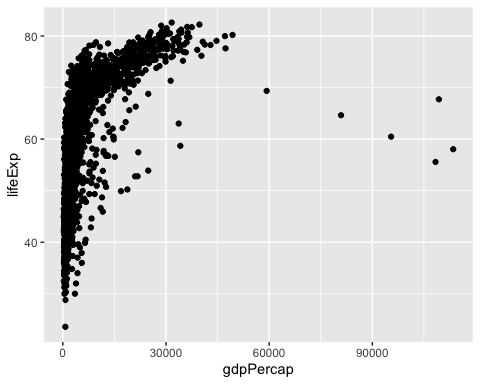
\includegraphics{w5_exercises_stats_and_visualization_answers_files/figure-latex/unnamed-chunk-29-1.pdf}

\hypertarget{d-4}{%
\subsubsection{d}\label{d-4}}

Of course this boxplot is not very nice, as we've basically created a
boxplot of a multimodal distribution: the average weights depends on the
animal. It would therefore be nicer to look at the weights for each of
the animals seperately. Use \texttt{boxplot} with a \texttt{formula},
where you tell \texttt{R} that weight depends on the type of animal. Is
this better?

\textbf{Answer:}

\begin{Shaded}
\begin{Highlighting}[]
\KeywordTok{boxplot}\NormalTok{(weight }\OperatorTok{~}\StringTok{ }\NormalTok{my_animals)}
\end{Highlighting}
\end{Shaded}

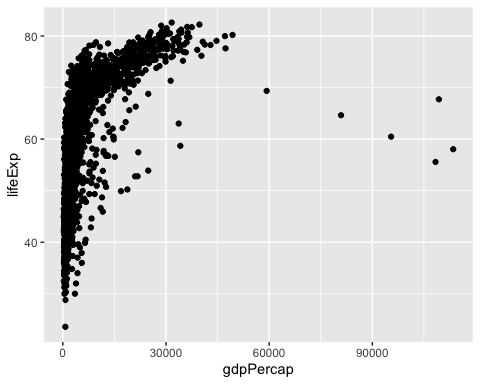
\includegraphics{w5_exercises_stats_and_visualization_answers_files/figure-latex/unnamed-chunk-30-1.pdf}
Better yes, but not perfect, as we don't see the distribution of weights
for the smaller animals very nicely. Better would be to also show those
seperately. E.g. using:

\begin{Shaded}
\begin{Highlighting}[]
\KeywordTok{boxplot}\NormalTok{(weight[my_animals}\OperatorTok\KeywordTok{c}\NormalTok{(}\StringTok{"cat"}\NormalTok{, }\StringTok{"dog"}\NormalTok{)] }\OperatorTok{~}\StringTok{  }\NormalTok{my_animals[my_animals}\OperatorTok\KeywordTok{c}\NormalTok{(}\StringTok{"cat"}\NormalTok{, }\StringTok{"dog"}\NormalTok{)])}
\end{Highlighting}
\end{Shaded}

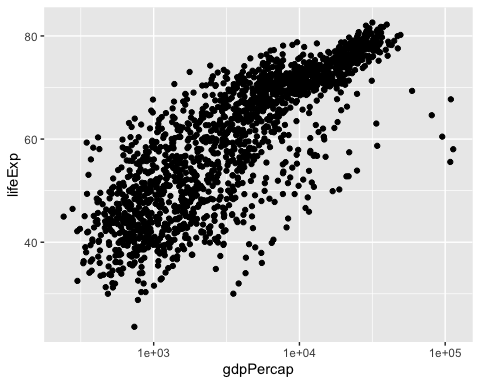
\includegraphics{w5_exercises_stats_and_visualization_answers_files/figure-latex/unnamed-chunk-31-1.pdf}

\newpage

\hypertarget{exercises-part-2}{%
\section{Exercises part 2}\label{exercises-part-2}}

\hypertarget{making-our-own-qqchisq-plot}{%
\subsection{2.1 Making our own qqchisq
plot}\label{making-our-own-qqchisq-plot}}

As discussed during the lecture, a QQ-plot compares (estimates of)
empericial quantiles with theoretical quantiles. In this exercise we
will make our own QQ-plot function.

Take the following random variable \texttt{x} as an example.

\begin{Shaded}
\begin{Highlighting}[]
\KeywordTok{set.seed}\NormalTok{(}\DecValTok{20171004}\NormalTok{)}
\NormalTok{x <-}\StringTok{ }\KeywordTok{rchisq}\NormalTok{(}\DecValTok{500}\NormalTok{, }\DataTypeTok{df =} \DecValTok{3}\NormalTok{)}
\end{Highlighting}
\end{Shaded}

\hypertarget{a-5}{%
\subsubsection{a}\label{a-5}}

Sort \texttt{x}.

\textbf{Answer:}

\begin{Shaded}
\begin{Highlighting}[]
\NormalTok{x <-}\StringTok{ }\KeywordTok{sort}\NormalTok{(x)}
\end{Highlighting}
\end{Shaded}

\hypertarget{b-5}{%
\subsubsection{b}\label{b-5}}

Produce a vector, called \texttt{t\_probs}, of length \(N\), where \(N\)
is the number of observations in \(X\), with a sequence from \(0.5/N\)
to \((N-0.5)/N\) with a stepsize of \(1/N\).

\textbf{Answer:}

\begin{Shaded}
\begin{Highlighting}[]
\NormalTok{N <-}\StringTok{ }\KeywordTok{length}\NormalTok{(x)}
\NormalTok{t_probs <-}\StringTok{ }\KeywordTok{seq}\NormalTok{(}\FloatTok{0.5}\NormalTok{, (N }\OperatorTok{-}\StringTok{ }\FloatTok{0.5}\NormalTok{), }\DataTypeTok{by =} \DecValTok{1}\NormalTok{)}\OperatorTok{/}\NormalTok{N}
\end{Highlighting}
\end{Shaded}

\hypertarget{c-6}{%
\subsubsection{c}\label{c-6}}

Turn \texttt{t\_probs} into values such that the cumulative
probabilities correspond with quantiles of a chisquare distribution with
degrees of freedom equal to \(3\).

\textbf{Answer:}

\begin{Shaded}
\begin{Highlighting}[]
\NormalTok{quantiles <-}\StringTok{ }\KeywordTok{qchisq}\NormalTok{(t_probs, }\DataTypeTok{df =} \DecValTok{3}\NormalTok{)}
\end{Highlighting}
\end{Shaded}

\hypertarget{d-5}{%
\subsubsection{d}\label{d-5}}

Plot the observed values \texttt{x} against the theoretical quantiles
obtained in \textbf{c}. Draw a line with unit slope and no intercept.
Would you say, from this plot, that the data is distributed similarly to
the theoritical distribution we considered?

\textbf{Answer:}

\begin{Shaded}
\begin{Highlighting}[]
\KeywordTok{plot}\NormalTok{(quantiles, x)}
\KeywordTok{abline}\NormalTok{(}\DataTypeTok{a =} \DecValTok{0}\NormalTok{, }\DataTypeTok{b =} \DecValTok{1}\NormalTok{, }\DataTypeTok{col =} \StringTok{'red'}\NormalTok{)}
\end{Highlighting}
\end{Shaded}

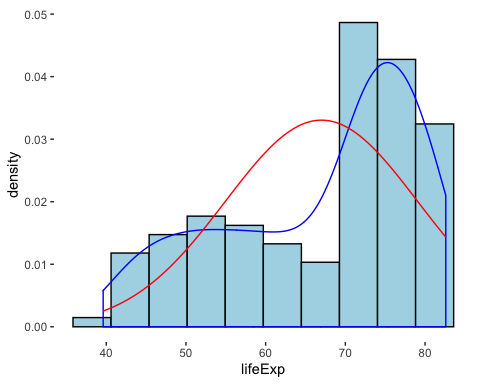
\includegraphics{w5_exercises_stats_and_visualization_answers_files/figure-latex/unnamed-chunk-36-1.pdf}

\hypertarget{e-2}{%
\subsubsection{e}\label{e-2}}

Look at the helpfile of \texttt{qqplot} and create a QQ-plot for a
chisquare distribution using the code from the example. Are there any
differences betweem the plot we made, and the plot of the example
(besides aesthetical stuff, such as a plot title)?

\textbf{Answer:}

\begin{Shaded}
\begin{Highlighting}[]
\CommentTok{## Q-Q plot for Chi^2 data against true theoretical distribution:}
\NormalTok{y <-}\StringTok{ }\NormalTok{x}
\KeywordTok{qqplot}\NormalTok{(}\KeywordTok{qchisq}\NormalTok{(}\KeywordTok{ppoints}\NormalTok{(}\DecValTok{500}\NormalTok{), }\DataTypeTok{df =} \DecValTok{3}\NormalTok{), y,}
       \DataTypeTok{main =} \KeywordTok{expression}\NormalTok{(}\StringTok{"Q-Q plot for"} \OperatorTok{~}\ErrorTok{~}\StringTok{ }\NormalTok{\{chi}\OperatorTok{^}\DecValTok{2}\NormalTok{\}[nu }\OperatorTok{==}\StringTok{ }\DecValTok{3}\NormalTok{]))}
\KeywordTok{qqline}\NormalTok{(y, }\DataTypeTok{distribution =} \ControlFlowTok{function}\NormalTok{(p) }\KeywordTok{qchisq}\NormalTok{(p, }\DataTypeTok{df =} \DecValTok{3}\NormalTok{),}
       \DataTypeTok{prob =} \KeywordTok{c}\NormalTok{(}\FloatTok{0.1}\NormalTok{, }\FloatTok{0.6}\NormalTok{), }\DataTypeTok{col =} \DecValTok{2}\NormalTok{)}
\KeywordTok{mtext}\NormalTok{(}\StringTok{"qqline(*, dist = qchisq(., df=3), prob = c(0.1, 0.6))"}\NormalTok{)}
\end{Highlighting}
\end{Shaded}

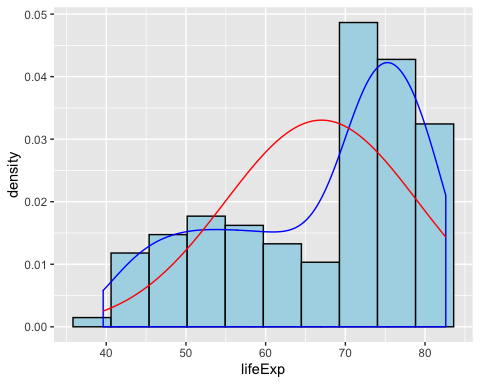
\includegraphics{w5_exercises_stats_and_visualization_answers_files/figure-latex/unnamed-chunk-37-1.pdf}
\texttt{qqline} creates a different line: one that goes through the
0.25th and 0.75th quartiles.

\hypertarget{outro}{%
\subsection{Outro}\label{outro}}

You may have noticed in \textbf{e} that \texttt{R} has a different
convention when it comes to drawing a \texttt{qqline}. It draws a line
that passes through the 0.25th, and 0.75th quartiles. This is a more
robust way of drawing the line, without need to rescale the line in case
of data that looks slightly different. For example redraw values for
\texttt{x} using:

\begin{Shaded}
\begin{Highlighting}[]
\KeywordTok{set.seed}\NormalTok{(}\DecValTok{20171004}\NormalTok{)}
\NormalTok{x <-}\StringTok{ }\KeywordTok{rchisq}\NormalTok{(}\DecValTok{500}\NormalTok{, }\DataTypeTok{df =} \DecValTok{3}\NormalTok{) }\OperatorTok{+}\StringTok{ }\DecValTok{3}
\end{Highlighting}
\end{Shaded}

and go through your plotting procedures again. Do you see that the line
is shifted, compared to the data? This is usually `easily' fixed, but a
more simple way is to just simply draw the \texttt{qqline} always
through the 0.25th and 0.75th quartiles. (In this course, both styles
are fine! Just be aware of it!)

\hypertarget{looking-into-sampling-distributions}{%
\subsection{2.2 Looking into sampling
distributions}\label{looking-into-sampling-distributions}}

In this exercise we will take a closer look at sampling distributions,
and the relationship between the variance of a sample, and the variance
of a sample mean. The relation is given by:
\(var(\bar{X}) = \frac{var(X)}{N}\).

For some extra info/recap view, for example, the first part of this
\href{https://www.youtube.com/watch?v=q50GpTdFYyI}{video} (until 4:12).
You may also want to take a look at:
\url{http://onlinestatbook.com/2/estimation/mean.html}.

\hypertarget{a-6}{%
\subsubsection{a}\label{a-6}}

Generate many samples, e.g 734, of size \(100\) (\(N = 100\)) where each
sample is i.i.d. according to a normal distribution with \(\mu = 2\) and
\(\sigma = 3\). Repeat this for samples with \(N = 10\) and
\(N = 1000\). Take \texttt{set.seed(1212)}. Show in R, with computations
on the generated samples, that the relation between sample variance and
sample mean variance holds. Think for a second about the strenght of
your evidence upon which you base your conclusions.

\textbf{Answer:}

\begin{Shaded}
\begin{Highlighting}[]
\KeywordTok{set.seed}\NormalTok{(}\DecValTok{1212}\NormalTok{)}
\NormalTok{B <-}\StringTok{ }\DecValTok{734}

\NormalTok{N <-}\StringTok{ }\DecValTok{10}
\NormalTok{N10 <-}\StringTok{ }\KeywordTok{replicate}\NormalTok{(B, }\KeywordTok{mean}\NormalTok{(}\KeywordTok{rnorm}\NormalTok{(N, }\DataTypeTok{mean =} \DecValTok{2}\NormalTok{, }\DataTypeTok{sd =} \DecValTok{3}\NormalTok{)))}

\NormalTok{N <-}\StringTok{ }\DecValTok{100}
\NormalTok{N100 <-}\StringTok{ }\KeywordTok{replicate}\NormalTok{(B, }\KeywordTok{mean}\NormalTok{(}\KeywordTok{rnorm}\NormalTok{(N, }\DataTypeTok{mean =} \DecValTok{2}\NormalTok{, }\DataTypeTok{sd =} \DecValTok{3}\NormalTok{)))}

\NormalTok{N <-}\StringTok{ }\DecValTok{1000}
\NormalTok{N1000 <-}\StringTok{ }\KeywordTok{replicate}\NormalTok{(B, }\KeywordTok{mean}\NormalTok{(}\KeywordTok{rnorm}\NormalTok{(N, }\DataTypeTok{mean =} \DecValTok{2}\NormalTok{, }\DataTypeTok{sd =} \DecValTok{3}\NormalTok{)))}

\KeywordTok{sd}\NormalTok{(N10) }\OperatorTok{*}\StringTok{ }\KeywordTok{sqrt}\NormalTok{(}\DecValTok{10}\NormalTok{)}
\end{Highlighting}
\end{Shaded}

\begin{verbatim}
## [1] 3.12486
\end{verbatim}

\begin{Shaded}
\begin{Highlighting}[]
\KeywordTok{sd}\NormalTok{(N100) }\OperatorTok{*}\StringTok{ }\KeywordTok{sqrt}\NormalTok{(}\DecValTok{100}\NormalTok{)}
\end{Highlighting}
\end{Shaded}

\begin{verbatim}
## [1] 3.047378
\end{verbatim}

\begin{Shaded}
\begin{Highlighting}[]
\KeywordTok{sd}\NormalTok{(N1000) }\OperatorTok{*}\StringTok{ }\KeywordTok{sqrt}\NormalTok{(}\DecValTok{1000}\NormalTok{)}
\end{Highlighting}
\end{Shaded}

\begin{verbatim}
## [1] 2.985925
\end{verbatim}

\hypertarget{b-6}{%
\subsubsection{b}\label{b-6}}

Instead of expression the relationship in numbers (as in one of the
previous exercises), we now want to express it using some visualization.
Do this in the following two ways:

\begin{enumerate}
\def\labelenumi{\alph{enumi})}
\tightlist
\item
  by visualizing the sampling distributions of the mean for the samples
  with the three different sample sizes generated for question 1 (you
  may show three separate plots)
\item
  by computing the 95\(\%\) confidence intervals of the mean for three
  samples picked from the samples you generated for question 1 (i.e.,
  one sample with \(N = 10\), one with \(N = 100\) and one with
  \(N = 1000\)). Assume in the computation of the confidence interval,
  that you do not know \(\sigma\), thus you have to use the sample
  estimate of it (\(s\)). Furthermore, make use of the
  \(t\)-distribution for choosing the values of \(t\) to be used in a
  confidence interval. In R, you can obtain these \(t\)-values using the
  function \texttt{qt()}. For example, the values for a sample size of
  \(n = 5\) are obtained by \texttt{qt(c(.025,\ .975),\ df\ =\ 4)}.
\end{enumerate}

\textbf{Answer:}

\begin{Shaded}
\begin{Highlighting}[]
\KeywordTok{hist}\NormalTok{(N10)}
\end{Highlighting}
\end{Shaded}

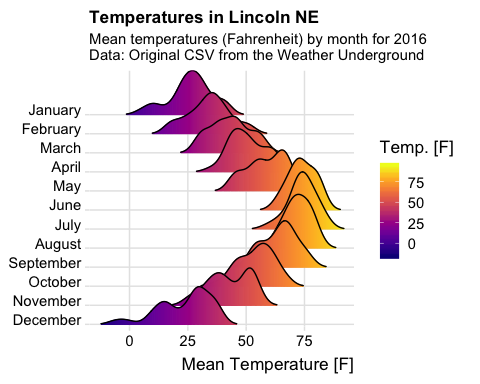
\includegraphics{w5_exercises_stats_and_visualization_answers_files/figure-latex/unnamed-chunk-40-1.pdf}

\begin{Shaded}
\begin{Highlighting}[]
\KeywordTok{hist}\NormalTok{(N100)}
\end{Highlighting}
\end{Shaded}

\includegraphics{w5_exercises_stats_and_visualization_answers_files/figure-latex/unnamed-chunk-40-2.pdf}

\begin{Shaded}
\begin{Highlighting}[]
\KeywordTok{hist}\NormalTok{(N1000)}
\end{Highlighting}
\end{Shaded}

\includegraphics{w5_exercises_stats_and_visualization_answers_files/figure-latex/unnamed-chunk-40-3.pdf}

\begin{Shaded}
\begin{Highlighting}[]
\NormalTok{limits_N10 <-}\StringTok{ }\KeywordTok{qt}\NormalTok{(}\KeywordTok{c}\NormalTok{(}\FloatTok{0.025}\NormalTok{, }\FloatTok{0.975}\NormalTok{), }\DataTypeTok{df =} \DecValTok{9}\NormalTok{)}
\NormalTok{limits_N100 <-}\StringTok{ }\KeywordTok{qt}\NormalTok{(}\KeywordTok{c}\NormalTok{(}\FloatTok{0.025}\NormalTok{, }\FloatTok{0.975}\NormalTok{), }\DataTypeTok{df =} \DecValTok{99}\NormalTok{)}
\NormalTok{limits_N1000 <-}\StringTok{ }\KeywordTok{qt}\NormalTok{(}\KeywordTok{c}\NormalTok{(}\FloatTok{0.025}\NormalTok{, }\FloatTok{0.975}\NormalTok{), }\DataTypeTok{df =} \DecValTok{999}\NormalTok{)}

\KeywordTok{mean}\NormalTok{(N10) }\OperatorTok{+}\StringTok{ }\NormalTok{limits_N10 }\OperatorTok{*}\StringTok{ }\KeywordTok{sd}\NormalTok{(N10)}
\end{Highlighting}
\end{Shaded}

\begin{verbatim}
## [1] -0.2590674  4.2117133
\end{verbatim}

\begin{Shaded}
\begin{Highlighting}[]
\KeywordTok{mean}\NormalTok{(N100) }\OperatorTok{+}\StringTok{ }\NormalTok{limits_N100 }\OperatorTok{*}\StringTok{ }\KeywordTok{sd}\NormalTok{(N100)}
\end{Highlighting}
\end{Shaded}

\begin{verbatim}
## [1] 1.379963 2.589295
\end{verbatim}

\begin{Shaded}
\begin{Highlighting}[]
\KeywordTok{mean}\NormalTok{(N1000) }\OperatorTok{+}\StringTok{ }\NormalTok{limits_N1000 }\OperatorTok{*}\StringTok{ }\KeywordTok{sd}\NormalTok{(N1000)}
\end{Highlighting}
\end{Shaded}

\begin{verbatim}
## [1] 1.811918 2.182500
\end{verbatim}

\hypertarget{c-7}{%
\subsubsection{c}\label{c-7}}

Write a function in \texttt{R} that computes the mean and its 95\(\%\)
confidence interval of a variable. The input argument of the function is
a vector that can have different lengths. The output is a list with two
components: the mean, and the 95\(\%\) confidence interval.

\textbf{Answer:}

\begin{Shaded}
\begin{Highlighting}[]
\NormalTok{CI <-}\StringTok{ }\ControlFlowTok{function}\NormalTok{(x)\{}
\NormalTok{  N <-}\StringTok{ }\KeywordTok{length}\NormalTok{(x)}
\NormalTok{  limits <-}\StringTok{ }\KeywordTok{qt}\NormalTok{(}\KeywordTok{c}\NormalTok{(}\FloatTok{0.025}\NormalTok{, }\FloatTok{0.975}\NormalTok{), }\DataTypeTok{df =}\NormalTok{ N }\OperatorTok{-}\StringTok{ }\DecValTok{1}\NormalTok{)}
\NormalTok{  mean <-}\StringTok{ }\KeywordTok{mean}\NormalTok{(x)}
  
  \KeywordTok{return}\NormalTok{(}\KeywordTok{list}\NormalTok{(}
    \DataTypeTok{mean =}\NormalTok{ mean, }
    \DataTypeTok{ci =}\NormalTok{ mean }\OperatorTok{+}\StringTok{ }\NormalTok{limits }\OperatorTok{*}\StringTok{ }\KeywordTok{sd}\NormalTok{(x)}
\NormalTok{  ))}
\NormalTok{\}}
\KeywordTok{CI}\NormalTok{(N1000)}
\end{Highlighting}
\end{Shaded}

\begin{verbatim}
## $mean
## [1] 1.997209
## 
## $ci
## [1] 1.811837 2.182581
\end{verbatim}

\hypertarget{contour-visualizing-a-pyramid}{%
\subsection{2.3 Contour: visualizing a
pyramid}\label{contour-visualizing-a-pyramid}}

In this exercise we'll visualize a pyramid, using a 2D plot. Of course
you all know what a pyramid looks like, but if you're unsure, go to the
library and look in some history textbooks. Hopefully, using such a
simple shape will give you some insight in how to read a
\texttt{contour}plot, and how to create one.

\hypertarget{a-7}{%
\subsubsection{a}\label{a-7}}

Create a 15 by 15 matrix. Fill the outer ring of values with a 1, fill
the second ring from outside with a 2, etc. These value indicate the
`height' of the pyramid at that point.

Here's some cody to create a 5 by 5 matrix as an example:

\begin{Shaded}
\begin{Highlighting}[]
\NormalTok{nrow <-}\StringTok{ }\DecValTok{5}
\NormalTok{ncol <-}\StringTok{ }\DecValTok{5}
\NormalTok{pyramid <-}\StringTok{ }\KeywordTok{matrix}\NormalTok{(}\DecValTok{0}\NormalTok{, }\DataTypeTok{nrow=}\NormalTok{nrow, }\DataTypeTok{ncol=}\NormalTok{ncol)}
\ControlFlowTok{for}\NormalTok{ (i }\ControlFlowTok{in} \DecValTok{1}\OperatorTok{:}\NormalTok{nrow)\{}
  \ControlFlowTok{for}\NormalTok{ (j }\ControlFlowTok{in} \DecValTok{1}\OperatorTok{:}\NormalTok{ncol)\{}
\NormalTok{    pyramid[i, j] <-}\StringTok{ }\KeywordTok{min}\NormalTok{(}\KeywordTok{min}\NormalTok{(i, nrow}\OperatorTok{-}\NormalTok{i}\OperatorTok{+}\DecValTok{1}\NormalTok{), }\KeywordTok{min}\NormalTok{(j, ncol}\OperatorTok{-}\NormalTok{j}\OperatorTok{+}\DecValTok{1}\NormalTok{))}
\NormalTok{  \}}
\NormalTok{\}}

\CommentTok{# look at the contents:}
\NormalTok{pyramid}
\end{Highlighting}
\end{Shaded}

\begin{verbatim}
##      [,1] [,2] [,3] [,4] [,5]
## [1,]    1    1    1    1    1
## [2,]    1    2    2    2    1
## [3,]    1    2    3    2    1
## [4,]    1    2    2    2    1
## [5,]    1    1    1    1    1
\end{verbatim}

\textbf{Answer:}

\begin{Shaded}
\begin{Highlighting}[]
\NormalTok{nrow <-}\StringTok{ }\DecValTok{15}
\NormalTok{ncol <-}\StringTok{ }\DecValTok{15}
\NormalTok{pyramid <-}\StringTok{ }\KeywordTok{matrix}\NormalTok{(}\DecValTok{0}\NormalTok{, }\DataTypeTok{nrow=}\NormalTok{nrow, }\DataTypeTok{ncol=}\NormalTok{ncol)}
\ControlFlowTok{for}\NormalTok{ (i }\ControlFlowTok{in} \DecValTok{1}\OperatorTok{:}\NormalTok{nrow)\{}
  \ControlFlowTok{for}\NormalTok{ (j }\ControlFlowTok{in} \DecValTok{1}\OperatorTok{:}\NormalTok{ncol)\{}
\NormalTok{    pyramid[i, j] <-}\StringTok{ }\KeywordTok{min}\NormalTok{(}\KeywordTok{min}\NormalTok{(i, nrow}\OperatorTok{-}\NormalTok{i}\OperatorTok{+}\DecValTok{1}\NormalTok{), }\KeywordTok{min}\NormalTok{(j, ncol}\OperatorTok{-}\NormalTok{j}\OperatorTok{+}\DecValTok{1}\NormalTok{))}
\NormalTok{  \}}
\NormalTok{\}}

\CommentTok{# look at the contents:}
\NormalTok{pyramid}
\end{Highlighting}
\end{Shaded}

\begin{verbatim}
##       [,1] [,2] [,3] [,4] [,5] [,6] [,7] [,8] [,9] [,10] [,11] [,12] [,13]
##  [1,]    1    1    1    1    1    1    1    1    1     1     1     1     1
##  [2,]    1    2    2    2    2    2    2    2    2     2     2     2     2
##  [3,]    1    2    3    3    3    3    3    3    3     3     3     3     3
##  [4,]    1    2    3    4    4    4    4    4    4     4     4     4     3
##  [5,]    1    2    3    4    5    5    5    5    5     5     5     4     3
##  [6,]    1    2    3    4    5    6    6    6    6     6     5     4     3
##  [7,]    1    2    3    4    5    6    7    7    7     6     5     4     3
##  [8,]    1    2    3    4    5    6    7    8    7     6     5     4     3
##  [9,]    1    2    3    4    5    6    7    7    7     6     5     4     3
## [10,]    1    2    3    4    5    6    6    6    6     6     5     4     3
## [11,]    1    2    3    4    5    5    5    5    5     5     5     4     3
## [12,]    1    2    3    4    4    4    4    4    4     4     4     4     3
## [13,]    1    2    3    3    3    3    3    3    3     3     3     3     3
## [14,]    1    2    2    2    2    2    2    2    2     2     2     2     2
## [15,]    1    1    1    1    1    1    1    1    1     1     1     1     1
##       [,14] [,15]
##  [1,]     1     1
##  [2,]     2     1
##  [3,]     2     1
##  [4,]     2     1
##  [5,]     2     1
##  [6,]     2     1
##  [7,]     2     1
##  [8,]     2     1
##  [9,]     2     1
## [10,]     2     1
## [11,]     2     1
## [12,]     2     1
## [13,]     2     1
## [14,]     2     1
## [15,]     1     1
\end{verbatim}

\hypertarget{b-7}{%
\subsubsection{b}\label{b-7}}

Use \texttt{contour} to visualize the pyramid.What is used to represent
the height of the pyramid at each point?

\textbf{Answer:}

\begin{Shaded}
\begin{Highlighting}[]
\KeywordTok{contour}\NormalTok{(}\DataTypeTok{x=}\DecValTok{1}\OperatorTok{:}\NormalTok{nrow, }\DataTypeTok{y=}\DecValTok{1}\OperatorTok{:}\NormalTok{ncol, }\DataTypeTok{z=}\NormalTok{pyramid, }\DataTypeTok{nlevels=}\KeywordTok{length}\NormalTok{(}\KeywordTok{unique}\NormalTok{(}\KeywordTok{c}\NormalTok{(pyramid))))}
\end{Highlighting}
\end{Shaded}

\includegraphics{w5_exercises_stats_and_visualization_answers_files/figure-latex/unnamed-chunk-44-1.pdf}
Height lines! Like an old school map!

\hypertarget{c-8}{%
\subsubsection{c}\label{c-8}}

Use \texttt{image} to visualize the pyramid. What is used to represent
the height of the pyramid at each point?

\textbf{Answer:}

\begin{Shaded}
\begin{Highlighting}[]
\KeywordTok{image}\NormalTok{(pyramid)}
\end{Highlighting}
\end{Shaded}

\includegraphics{w5_exercises_stats_and_visualization_answers_files/figure-latex/unnamed-chunk-45-1.pdf}
The colour of course!

\hypertarget{make-a-heat-map-and-save-the-plot-as-.pdf}{%
\subsection{\texorpdfstring{2.4 Make a heat map and save the plot as
\texttt{.pdf}}{2.4 Make a heat map and save the plot as .pdf}}\label{make-a-heat-map-and-save-the-plot-as-.pdf}}

Take a look at the following link:
\href{http://flowingdata.com/2010/01/21/how-to-make-a-heatmap-a-quick-and-easy-solution/}{heatmap}.
Follow the coding instructions on the website. You can find the data
(\texttt{ppg2008.csv}) on the website, or in the \texttt{data} folder.
Save the final heatmap as a \texttt{.pdf} file.

\textbf{Answer:}

\begin{Shaded}
\begin{Highlighting}[]
\NormalTok{nba <-}\StringTok{ }\KeywordTok{read.csv}\NormalTok{(}\StringTok{"http://datasets.flowingdata.com/ppg2008.csv"}\NormalTok{, }\DataTypeTok{sep=}\StringTok{","}\NormalTok{)}
\KeywordTok{row.names}\NormalTok{(nba) <-}\StringTok{ }\NormalTok{nba}\OperatorTok{$}\NormalTok{Name}
\NormalTok{nba <-}\StringTok{ }\NormalTok{nba[,}\DecValTok{2}\OperatorTok{:}\DecValTok{20}\NormalTok{]}
\NormalTok{nba_matrix <-}\StringTok{ }\KeywordTok{data.matrix}\NormalTok{(nba)}
\KeywordTok{pdf}\NormalTok{(}\StringTok{"0_images/nba_heatmap.pdf"}\NormalTok{)}
\NormalTok{nba_heatmap <-}\StringTok{ }\KeywordTok{heatmap}\NormalTok{(}
\NormalTok{  nba_matrix, }\DataTypeTok{Rowv=}\OtherTok{NA}\NormalTok{, }\DataTypeTok{Colv=}\OtherTok{NA}\NormalTok{, }\DataTypeTok{col =} \KeywordTok{cm.colors}\NormalTok{(}\DecValTok{256}\NormalTok{), }
  \DataTypeTok{scale=}\StringTok{"column"}\NormalTok{, }\DataTypeTok{margins=}\KeywordTok{c}\NormalTok{(}\DecValTok{5}\NormalTok{,}\DecValTok{10}\NormalTok{))}
\KeywordTok{dev.off}\NormalTok{()}
\end{Highlighting}
\end{Shaded}

\begin{verbatim}
## pdf 
##   2
\end{verbatim}

\newpage

\hypertarget{self-study}{%
\section{3 Self-study}\label{self-study}}

\hypertarget{visualizing-a-bivariate-normal-density}{%
\subsection{3.1 Visualizing a bivariate normal
density}\label{visualizing-a-bivariate-normal-density}}

Before you start this exercise, install the package \texttt{mvtnorm}.

\hypertarget{a-8}{%
\subsubsection{a}\label{a-8}}

Take a look at \texttt{dmvnorm} in the \texttt{mvtnorm} package. To
calculate the density function of a bivariate normal distribution, you
will need the covariance matrix of the distribution. Create one, where
both marginal distributions are standard normally distributed, and are
correlated with a coefficient of 0.7.

\textbf{Answer:}

\begin{Shaded}
\begin{Highlighting}[]
\NormalTok{sigma_cor <-}\StringTok{ }\KeywordTok{matrix}\NormalTok{(}\KeywordTok{c}\NormalTok{(}\DecValTok{1}\NormalTok{, }\FloatTok{0.7}\NormalTok{, }\FloatTok{0.7}\NormalTok{, }\DecValTok{1}\NormalTok{), }\DataTypeTok{ncol=}\DecValTok{2}\NormalTok{)}
\end{Highlighting}
\end{Shaded}

\hypertarget{b-8}{%
\subsubsection{b}\label{b-8}}

Take a look at \texttt{expand.grid}. Use it to create quantiles, so you
can evaluate the bivariate normal density at many points. For example at
\texttt{x1\ =\ -3}, and \texttt{x2\ =\ 0}, or \texttt{x1\ =\ -3}, and
\texttt{x2\ =\ 1}, etc. You will need many points (e.g.~many
combinations of values of \texttt{x1} and \texttt{x2}) to get a nice
picture of the density.

\textbf{Answer:}

\begin{Shaded}
\begin{Highlighting}[]
\NormalTok{quantiles_seq <-}\StringTok{ }\KeywordTok{seq}\NormalTok{(}\OperatorTok{-}\DecValTok{3}\NormalTok{, }\DecValTok{3}\NormalTok{, }\DataTypeTok{by =} \FloatTok{0.1}\NormalTok{)}
\NormalTok{quantiles <-}\StringTok{ }\KeywordTok{expand.grid}\NormalTok{(quantiles_seq, quantiles_seq)}
\end{Highlighting}
\end{Shaded}

\hypertarget{c.}{%
\subsubsection{c.}\label{c.}}

Put the quantiles you've created into \texttt{dmvnorm} twice, once with
all the defaults, and once also providing the covariance matrix you
created in \textbf{a}. Save the results of both operations.

\textbf{Answer:}

\begin{Shaded}
\begin{Highlighting}[]
\KeywordTok{library}\NormalTok{(mvtnorm)}
\NormalTok{densities_uncor <-}\StringTok{ }\KeywordTok{dmvnorm}\NormalTok{(quantiles)}
\NormalTok{densities_cor <-}\StringTok{ }\KeywordTok{dmvnorm}\NormalTok{(quantiles, }\DataTypeTok{sigma =}\NormalTok{ sigma_cor)}
\end{Highlighting}
\end{Shaded}

\hypertarget{d.}{%
\subsubsection{d.}\label{d.}}

If we want to use \texttt{contour}, we need to put the density values
into a matrix. The entries in this matrix represent a grid, with density
evaluations at the intersections of the gridlines. An important issue is
that we need to make sure the ordering of the values is correct:
e.g.~the value in the second row, and third column (where grid lines for
row two and column three meet), needs to be the value of evaluating the
second quantile for the first normal variable and the third quantile for
the second normal variable.

Convert the quantiles you've created into such a matrix now.

\textbf{Answer:}

\begin{Shaded}
\begin{Highlighting}[]
\KeywordTok{head}\NormalTok{(quantiles)}
\end{Highlighting}
\end{Shaded}

\begin{verbatim}
##   Var1 Var2
## 1 -3.0   -3
## 2 -2.9   -3
## 3 -2.8   -3
## 4 -2.7   -3
## 5 -2.6   -3
## 6 -2.5   -3
\end{verbatim}

\begin{Shaded}
\begin{Highlighting}[]
\CommentTok{# in my case, for a single var2 quantile, all the quantiles of var1 are calculated}
\CommentTok{# this is as if we are in a single column of a matrix, and provide the row entries.}
\CommentTok{# so if we fill or matrix by columns, the various values of var1 will correspond to the rows}
\CommentTok{# and the various values of var2 will correspond to the columns}
\NormalTok{densities_uncor_matrix <-}\StringTok{ }\KeywordTok{matrix}\NormalTok{(densities_uncor, }\DataTypeTok{ncol =} \KeywordTok{sqrt}\NormalTok{(}\KeywordTok{length}\NormalTok{(densities_uncor)))}
\NormalTok{densities_cor_matrix <-}\StringTok{ }\KeywordTok{matrix}\NormalTok{(densities_cor, }\DataTypeTok{ncol =} \KeywordTok{sqrt}\NormalTok{(}\KeywordTok{length}\NormalTok{(densities_cor)))}
\end{Highlighting}
\end{Shaded}

\hypertarget{e.}{%
\subsubsection{e.}\label{e.}}

You now have all the ingredients you need for \texttt{contour}. Make a
contourplot of both bivariate normal distributions. Do they look the
same? What's the big difference?

\textbf{Answer:}

\begin{Shaded}
\begin{Highlighting}[]
\KeywordTok{contour}\NormalTok{(}\DataTypeTok{x =}\NormalTok{ quantiles_seq, }\DataTypeTok{y =}\NormalTok{ quantiles_seq, }\DataTypeTok{z =}\NormalTok{ densities_uncor_matrix)}
\end{Highlighting}
\end{Shaded}

\includegraphics{w5_exercises_stats_and_visualization_answers_files/figure-latex/unnamed-chunk-51-1.pdf}

\begin{Shaded}
\begin{Highlighting}[]
\KeywordTok{contour}\NormalTok{(}\DataTypeTok{x =}\NormalTok{ quantiles_seq, }\DataTypeTok{y =}\NormalTok{ quantiles_seq, }\DataTypeTok{z =}\NormalTok{ densities_cor_matrix)}
\end{Highlighting}
\end{Shaded}

\includegraphics{w5_exercises_stats_and_visualization_answers_files/figure-latex/unnamed-chunk-51-2.pdf}

\hypertarget{hexbin}{%
\subsection{3.2 Hexbin}\label{hexbin}}

\textbf{we commented most of the plotting code as it takes forever to
plot and to show the plots in the pdf file, so uncomment or copy the
code if you want to check your answers!}

\hypertarget{a-9}{%
\subsubsection{a}\label{a-9}}

Read in the file \texttt{mystery.txt}. NB: it's a very big file, so this
might take a few seconds (the same goes for all the plotting you do
during this exercise).

\textbf{Answer:}

\begin{Shaded}
\begin{Highlighting}[]
\NormalTok{my_mystery <-}\StringTok{ }\KeywordTok{read.table}\NormalTok{(}\StringTok{"0_data/mystery.txt"}\NormalTok{)}
\end{Highlighting}
\end{Shaded}

\hypertarget{b-9}{%
\subsubsection{b}\label{b-9}}

Use some summary statistics functions on the data in the mystery file.
Make for example a histogram of \texttt{x} and \texttt{y}. Do you see
anything interesting?

\textbf{Answer:}

\begin{Shaded}
\begin{Highlighting}[]
\KeywordTok{summary}\NormalTok{(my_mystery)}
\end{Highlighting}
\end{Shaded}

\begin{verbatim}
##        x                  y          
##  Min.   :-0.50000   Min.   :-0.5000  
##  1st Qu.: 0.09759   1st Qu.: 0.3593  
##  Median : 0.48726   Median : 1.0465  
##  Mean   : 0.49020   Mean   : 1.0180  
##  3rd Qu.: 0.87762   3rd Qu.: 1.6866  
##  Max.   : 1.49998   Max.   : 2.5000
\end{verbatim}

\begin{Shaded}
\begin{Highlighting}[]
\KeywordTok{hist}\NormalTok{(my_mystery}\OperatorTok{$}\NormalTok{x)}
\end{Highlighting}
\end{Shaded}

\includegraphics{w5_exercises_stats_and_visualization_answers_files/figure-latex/unnamed-chunk-53-1.pdf}

\begin{Shaded}
\begin{Highlighting}[]
\KeywordTok{hist}\NormalTok{(my_mystery}\OperatorTok{$}\NormalTok{y)}
\end{Highlighting}
\end{Shaded}

\includegraphics{w5_exercises_stats_and_visualization_answers_files/figure-latex/unnamed-chunk-53-2.pdf}
Not really\ldots{}

\hypertarget{c-9}{%
\subsubsection{c}\label{c-9}}

The univariate stuff was boring. Let's now look at some bivariate stuff.
Are \texttt{x} and \texttt{y} correlated? Does a simple \texttt{plot} of
the entries show anything interesting?

\textbf{Answer:}

\begin{Shaded}
\begin{Highlighting}[]
\KeywordTok{cor}\NormalTok{(my_mystery)}
\end{Highlighting}
\end{Shaded}

\begin{verbatim}
##             x           y
## x 1.000000000 0.008873986
## y 0.008873986 1.000000000
\end{verbatim}

\begin{Shaded}
\begin{Highlighting}[]
\CommentTok{# plot(my_mystery)}
\end{Highlighting}
\end{Shaded}

Hmm\ldots{}. not really but that's probably due to the fact that we
can't see anything simply due to the sheer amount of observations.

\hypertarget{d-6}{%
\subsubsection{d}\label{d-6}}

Instead of \texttt{plot}, use \texttt{plot(hexbin())} from the
\texttt{hexbin} library. Play around with the argument \texttt{xbins}.
Do you see something interesting?

\textbf{Answer:}

\begin{Shaded}
\begin{Highlighting}[]
\KeywordTok{library}\NormalTok{(hexbin)}
\CommentTok{# plot(hexbin(my_mystery, xbins=100))}
\end{Highlighting}
\end{Shaded}

Clearly there's an R hidden in there!

\hypertarget{e-3}{%
\subsubsection{e}\label{e-3}}

Also try \texttt{smoothScatter}, you may want to play around with the
\texttt{bandwith} and the \texttt{nbin} arguments. Do you prefer
\texttt{hexbin} or \texttt{smoothScatter}?

\begin{Shaded}
\begin{Highlighting}[]
\CommentTok{# smoothScatter(my_mystery, bandwidth = 0.001, nbin=1000)}
\end{Highlighting}
\end{Shaded}

\texttt{smoothScatter} requires an extra argument we need to `tune', it
does provide more `smooth' plots though: the \texttt{hexbin} plot is, by
definition, a collection of hexagons, while \texttt{smoothScatter} can
take on more `fluid' shapes.

\hypertarget{sampling-from-a-triangle}{%
\subsection{3.4 Sampling from a
triangle}\label{sampling-from-a-triangle}}

During the lecture we've talked about how the cumulative distribution
function can be employed to produce random numbers from that
distribution. Look at the following density function:

\begin{itemize}
\tightlist
\item
  \(4x\), for \(x\in [0, 0.5)\)
\item
  \(4(1-x)\) for \(x\in [0.5, 1]\)
\end{itemize}

See an implementation below.

\begin{Shaded}
\begin{Highlighting}[]
\NormalTok{dtriangle <-}\StringTok{ }\ControlFlowTok{function}\NormalTok{(x)\{}
\NormalTok{  (x }\OperatorTok{>=}\StringTok{ }\DecValTok{0} \OperatorTok{&}\StringTok{ }\NormalTok{x }\OperatorTok{<}\StringTok{ }\FloatTok{0.5}\NormalTok{) }\OperatorTok{*}\StringTok{ }\DecValTok{4} \OperatorTok{*}\StringTok{ }\NormalTok{x }\OperatorTok{+}\StringTok{ }\NormalTok{(x }\OperatorTok{>=}\StringTok{ }\FloatTok{0.5} \OperatorTok{&}\StringTok{ }\NormalTok{x }\OperatorTok{<=}\StringTok{ }\DecValTok{1}\NormalTok{) }\OperatorTok{*}\StringTok{ }\DecValTok{4} \OperatorTok{*}\StringTok{ }\NormalTok{(}\DecValTok{1} \OperatorTok{-}\StringTok{ }\NormalTok{x)}
\NormalTok{\}}
\KeywordTok{curve}\NormalTok{(dtriangle, }\DataTypeTok{asp =} \DecValTok{1}\NormalTok{, }\DataTypeTok{from =} \FloatTok{-0.5}\NormalTok{, }\DataTypeTok{to =} \FloatTok{1.5}\NormalTok{)}
\end{Highlighting}
\end{Shaded}

\includegraphics{w5_exercises_stats_and_visualization_answers_files/figure-latex/unnamed-chunk-56-1.pdf}

\hypertarget{a-10}{%
\subsubsection{a}\label{a-10}}

Integrate the density of the triangle over its domain with
\texttt{integrate()}, is it a proper density function?

\textbf{Answer:}

\begin{Shaded}
\begin{Highlighting}[]
\KeywordTok{integrate}\NormalTok{(dtriangle, }\DataTypeTok{lower =} \DecValTok{-1}\NormalTok{, }\DataTypeTok{upper =} \DecValTok{2}\NormalTok{)}\OperatorTok{$}\NormalTok{value}
\end{Highlighting}
\end{Shaded}

\begin{verbatim}
## [1] 1
\end{verbatim}

Up to numerical error, yes.

\hypertarget{b-10}{%
\subsubsection{b}\label{b-10}}

Formulate a cumulative distribution function and write a function called
\texttt{ptriangle} that implements this. Note that besides integrating
the density function, you may also need to choose a proper constant,
such that the minimum of the function is \(0\), and the maximum is
\(1\).

\textbf{Answer:}

Integral (with properly chosen constant): * \(2x^2\), for
\(x\in [0, 0.5)\) * \(-2*(x+1)^2\) for \(x\in [0.5, 1]\)

\begin{Shaded}
\begin{Highlighting}[]
\NormalTok{y_var <-}\StringTok{ }\KeywordTok{sapply}\NormalTok{(}\KeywordTok{seq}\NormalTok{(}\DecValTok{0}\NormalTok{, }\DecValTok{1}\NormalTok{, }\DataTypeTok{by=}\FloatTok{0.01}\NormalTok{), }\ControlFlowTok{function}\NormalTok{(i) }\KeywordTok{integrate}\NormalTok{(dtriangle, }\DataTypeTok{lower=}\OperatorTok{-}\DecValTok{1}\NormalTok{, }\DataTypeTok{upper=}\NormalTok{i)}\OperatorTok{$}\NormalTok{value)}
\KeywordTok{plot}\NormalTok{(}
  \DataTypeTok{x =} \KeywordTok{seq}\NormalTok{(}\DecValTok{0}\NormalTok{, }\DecValTok{1}\NormalTok{, }\DataTypeTok{by=}\FloatTok{0.01}\NormalTok{), }
  \DataTypeTok{y =}\NormalTok{ y_var,}
  \DataTypeTok{ylab =} \StringTok{"CDF"}\NormalTok{, }\DataTypeTok{xlab =} \StringTok{"x"}
\NormalTok{)}
\NormalTok{ptriangle <-}\StringTok{ }\ControlFlowTok{function}\NormalTok{(x)\{}
\NormalTok{  (x }\OperatorTok{>=}\StringTok{ }\DecValTok{0} \OperatorTok{&}\StringTok{ }\NormalTok{x }\OperatorTok{<}\StringTok{ }\FloatTok{0.5}\NormalTok{) }\OperatorTok{*}\StringTok{ }\DecValTok{2} \OperatorTok{*}\StringTok{ }\NormalTok{x}\OperatorTok{^}\DecValTok{2} \OperatorTok{+}\StringTok{ }\NormalTok{(x }\OperatorTok{>=}\StringTok{ }\FloatTok{0.5} \OperatorTok{&}\StringTok{ }\NormalTok{x }\OperatorTok{<=}\StringTok{ }\DecValTok{1}\NormalTok{) }\OperatorTok{*}\StringTok{ }\NormalTok{(}\DecValTok{1} \OperatorTok{+}\StringTok{ }\DecValTok{-2} \OperatorTok{*}\StringTok{ }\NormalTok{(x}\DecValTok{-1}\NormalTok{)}\OperatorTok{^}\DecValTok{2}\NormalTok{) }\OperatorTok{+}\StringTok{ }\NormalTok{(x }\OperatorTok{>}\StringTok{ }\DecValTok{1}\NormalTok{)}
\NormalTok{\}}
\KeywordTok{curve}\NormalTok{(ptriangle, }\DataTypeTok{from=}\OperatorTok{-}\DecValTok{1}\NormalTok{, }\DataTypeTok{to=}\DecValTok{2}\NormalTok{, }\DataTypeTok{add=}\NormalTok{T, }\DataTypeTok{col=}\StringTok{'red'}\NormalTok{)}
\end{Highlighting}
\end{Shaded}

\includegraphics{w5_exercises_stats_and_visualization_answers_files/figure-latex/unnamed-chunk-58-1.pdf}

\hypertarget{c-10}{%
\subsubsection{c}\label{c-10}}

Formulate the inverse cumulative distribution function and write a
function called \texttt{qtriangle} that implements this.

\textbf{Answer:}

Inverse cumulative distribution: * \(4x\), for \(x\in [0, 0.5)\) *
\(4(1-x)\) for \(x\in [0.5, 1]\)

\begin{Shaded}
\begin{Highlighting}[]
\NormalTok{qtriangle <-}\StringTok{ }\ControlFlowTok{function}\NormalTok{(x)\{}
\NormalTok{  (x }\OperatorTok{>=}\StringTok{ }\DecValTok{0} \OperatorTok{&}\StringTok{ }\NormalTok{x }\OperatorTok{<}\StringTok{ }\FloatTok{0.5}\NormalTok{) }\OperatorTok{*}\StringTok{ }\KeywordTok{sqrt}\NormalTok{(x }\OperatorTok{/}\StringTok{ }\DecValTok{2}\NormalTok{) }\OperatorTok{+}\StringTok{ }\NormalTok{(x }\OperatorTok{>=}\StringTok{ }\FloatTok{0.5} \OperatorTok{&}\StringTok{ }\NormalTok{x }\OperatorTok{<=}\StringTok{ }\DecValTok{1}\NormalTok{) }\OperatorTok{*}\StringTok{ }\NormalTok{(}\DecValTok{1} \OperatorTok{-}\StringTok{ }\KeywordTok{sqrt}\NormalTok{((}\DecValTok{1} \OperatorTok{-}\StringTok{ }\NormalTok{x) }\OperatorTok{/}\StringTok{ }\DecValTok{2}\NormalTok{)) }\OperatorTok{+}\StringTok{ }\NormalTok{(x }\OperatorTok{>}\StringTok{ }\DecValTok{1}\NormalTok{)}
\NormalTok{\}}
\end{Highlighting}
\end{Shaded}

\hypertarget{d-7}{%
\subsubsection{d}\label{d-7}}

Write a function called \texttt{rtriangle} that samples \texttt{n}
random values from a triangle distribution.

\textbf{Answer:}

\begin{Shaded}
\begin{Highlighting}[]
\NormalTok{rtriangle <-}\StringTok{ }\ControlFlowTok{function}\NormalTok{(n)\{}
\NormalTok{  x <-}\StringTok{ }\KeywordTok{seq}\NormalTok{(}\DecValTok{0}\NormalTok{, }\DecValTok{1}\NormalTok{, }\DataTypeTok{length =}\NormalTok{ n)}
  \KeywordTok{return}\NormalTok{(}\KeywordTok{qtriangle}\NormalTok{(x))}
\NormalTok{\}}
\KeywordTok{hist}\NormalTok{(}\KeywordTok{rtriangle}\NormalTok{(}\FloatTok{1e4}\NormalTok{), }\DataTypeTok{breaks =} \StringTok{"FD"}\NormalTok{, }\DataTypeTok{col =} \StringTok{'lightblue'}\NormalTok{)}
\end{Highlighting}
\end{Shaded}

\includegraphics{w5_exercises_stats_and_visualization_answers_files/figure-latex/unnamed-chunk-60-1.pdf}

\hypertarget{coordinate-descent-for-advanced-students-only}{%
\subsection{3.5 Coordinate descent (For advanced students
only!)}\label{coordinate-descent-for-advanced-students-only}}

We've previously seen the Gradient descent algorithm (Week 4). A short
recap: there are various methods of estimating the parameters of a
statistical model e.g.~least squares or maximum likelihood estimation.
In maximum likelihood estimation a maximum of a real function (the
likelihood function) needs to be found by means of optimization. Various
optimization methods exist for finding the minimum or maximum of a real
function.

Like Gradient descent, Coordinate descent is an iterative algorithm,
that can be used to find a (local) minimum of a function that involves
more than \(1\) parameter! The idea is that one conditions on all
parameters except \(1\), update the parameter we did not condition on,
and repeat this for all parameters. We repeat this cycle many times
until convergence.

Take for example the function \(f(x, y) = x^2 + y^2 + x\cdot y)\). The
minimum can be found by condition on some \(x\) (keep it fixed) and find
the minimum for \(y\) given this value of \(x\). We then condition on
this new value of \(y\), and find a new \(x\) (the one that minimizes
\(f\), w.r.t. \(x\), given a value for \(y\)). We then repeat this until
the parameters \(x\) and \(y\) do not change in between updates.

\hypertarget{a-11}{%
\subsubsection{a}\label{a-11}}

Write an \texttt{R} function that uses the idea of coordinate descent to
find the minimum of a function of the form:

\(f(x, y) = ax^2 + by^2 + cx\cdot y\), with \(a\), \(b\) and \(c\) some
real numbers.

You will need:

\begin{itemize}
\tightlist
\item
  A function to evaluate the partial derivative w.r.t. \(x\), and solve
  for \(x\) s.t. \(f'_x(x, y | y) = 0\)
\item
  A function to evaluate the partial derivative w.r.t. \(y\), and solve
  for \(y\) s.t. \(f'_y(x, y | x) = 0\)
\item
  A while loop that repeats the update cycle until the sum of the
  absolute differences \(|x_{n+1} - x_{n}|\) and \(|y_{n+1} - y_{n}|\)
  is smaller than \texttt{1e-4}.
\end{itemize}

The input of the function should be a starting value for \(x\), a
starting value for \(y\), \(a\), \(b\), and \(c\). The output should be
a dataframe with an entry for the values of \(x\) and \(y\) at each step
of the algorithm. So the first entry of this dataframe is the starting
values, provided by you, of \(x\) and \(y\). The second entry is the
first value of \(y\), and the update of \(x\), given the current value
of \(y\). The third entry is the updated value of \(x\) and the update
value of \(y\). And so on.

Make sure that the algorithm performs no more than a \(100\) cycles of
updating both \(x\) and \(y\)

\textbf{Answer:}

\begin{Shaded}
\begin{Highlighting}[]
\CommentTok{#partial derivatives, w.r.t. x}
\NormalTok{SolveFx <-}\StringTok{ }\ControlFlowTok{function}\NormalTok{(y, a, c)\{}
  \KeywordTok{return}\NormalTok{(}\OperatorTok{-}\NormalTok{c}\OperatorTok{*}\NormalTok{y}\OperatorTok{/}\NormalTok{(}\DecValTok{2}\OperatorTok{*}\NormalTok{a))}
\NormalTok{\}}

\CommentTok{#partial derivative w.r.t. y}
\NormalTok{SolveFy <-}\StringTok{ }\ControlFlowTok{function}\NormalTok{(x, b, c)\{}
  \KeywordTok{return}\NormalTok{(}\OperatorTok{-}\NormalTok{c}\OperatorTok{*}\NormalTok{x}\OperatorTok{/}\NormalTok{(}\DecValTok{2}\OperatorTok{*}\NormalTok{b))}
\NormalTok{\}}

\NormalTok{CoordinateDescent <-}\StringTok{ }\ControlFlowTok{function}\NormalTok{(x0, y0, a, b, c)\{}
  
  \CommentTok{#start value for eps:}
\NormalTok{  eps <-}\StringTok{ }\OtherTok{Inf}
\NormalTok{  max.iter <-}\StringTok{ }\DecValTok{100}
  
\NormalTok{  x.vec <-}\StringTok{ }\KeywordTok{numeric}\NormalTok{(max.iter}\OperatorTok{*}\DecValTok{2}\NormalTok{)}
\NormalTok{  y.vec <-}\StringTok{ }\KeywordTok{numeric}\NormalTok{(max.iter}\OperatorTok{*}\DecValTok{2}\NormalTok{)}
  
\NormalTok{  counter <-}\StringTok{ }\DecValTok{1}
\NormalTok{  cycle <-}\StringTok{ }\DecValTok{1}
\NormalTok{  x.vec[counter] <-}\StringTok{ }\NormalTok{x0}
\NormalTok{  y.vec[counter] <-}\StringTok{ }\NormalTok{y0}
  
\NormalTok{  continue <-}\StringTok{ }\OtherTok{TRUE}
  \ControlFlowTok{while}\NormalTok{ (continue)\{}
    
\NormalTok{    x.vec[counter}\OperatorTok{+}\DecValTok{1}\NormalTok{] <-}\StringTok{ }\KeywordTok{SolveFx}\NormalTok{(y.vec[counter], a, c)}
\NormalTok{    y.vec[counter}\OperatorTok{+}\DecValTok{1}\NormalTok{] <-}\StringTok{ }\NormalTok{y.vec[counter]}
      
\NormalTok{    counter <-}\StringTok{ }\NormalTok{counter }\OperatorTok{+}\StringTok{ }\DecValTok{1}
    
\NormalTok{    x.vec[counter}\OperatorTok{+}\DecValTok{1}\NormalTok{] <-}\StringTok{ }\NormalTok{x.vec[counter]}
\NormalTok{    y.vec[counter}\OperatorTok{+}\DecValTok{1}\NormalTok{] <-}\StringTok{ }\KeywordTok{SolveFy}\NormalTok{(x.vec[counter], b, c)}
    
\NormalTok{    counter <-}\StringTok{ }\NormalTok{counter }\OperatorTok{+}\StringTok{ }\DecValTok{1}
    
\NormalTok{    eps <-}\StringTok{ }\KeywordTok{abs}\NormalTok{(x.vec[counter}\DecValTok{-1}\NormalTok{]}\OperatorTok{-}\NormalTok{x.vec[counter]) }\OperatorTok{+}\StringTok{ }\KeywordTok{abs}\NormalTok{(y.vec[counter}\DecValTok{-1}\NormalTok{] }\OperatorTok{-}\StringTok{ }\NormalTok{y.vec[counter])}
    
    \ControlFlowTok{if}\NormalTok{ (eps }\OperatorTok{<}\StringTok{ }\FloatTok{1e-4} \OperatorTok{|}\StringTok{ }\NormalTok{cycle }\OperatorTok{==}\StringTok{ }\NormalTok{max.iter)\{}
\NormalTok{      continue <-}\StringTok{ }\OtherTok{FALSE}
\NormalTok{    \}}
\NormalTok{    cycle <-}\StringTok{ }\NormalTok{cycle }\OperatorTok{+}\StringTok{ }\DecValTok{1}
\NormalTok{  \}}
  
\NormalTok{  update.history <-}\StringTok{ }\KeywordTok{data.frame}\NormalTok{(}\DataTypeTok{x =}\NormalTok{ x.vec[}\DecValTok{1}\OperatorTok{:}\NormalTok{counter], }\DataTypeTok{y=}\NormalTok{y.vec[}\DecValTok{1}\OperatorTok{:}\NormalTok{counter])}
  
  \KeywordTok{return}\NormalTok{(update.history)}
\NormalTok{\}}
\end{Highlighting}
\end{Shaded}

\hypertarget{b-11}{%
\subsubsection{b}\label{b-11}}

Demonstrate the algorithm for the function
\(g(x, y) = x^2 + 2y^2 - x\cdot y\) for start values \(x_0 = -3\) and
\(y_0 = -2\).

Make a contourplot of the function \(g\). Add to the contourplot, using
the function \texttt{segments}, a line between each subsequent update of
the parameters.

\textbf{Answer:}

\begin{Shaded}
\begin{Highlighting}[]
\NormalTok{f <-}\StringTok{ }\ControlFlowTok{function}\NormalTok{(x, y, a, b, c)\{}
\NormalTok{  a}\OperatorTok{*}\NormalTok{x}\OperatorTok{^}\DecValTok{2}\OperatorTok{+}\NormalTok{b}\OperatorTok{*}\NormalTok{y}\OperatorTok{^}\DecValTok{2}\OperatorTok{+}\NormalTok{c}\OperatorTok{*}\NormalTok{x}\OperatorTok{*}\NormalTok{y}
\NormalTok{\}}

\NormalTok{values <-}\StringTok{ }\KeywordTok{seq}\NormalTok{(}\OperatorTok{-}\DecValTok{3}\NormalTok{, }\DecValTok{3}\NormalTok{, }\DataTypeTok{by=}\FloatTok{0.1}\NormalTok{)}
\end{Highlighting}
\end{Shaded}

\begin{Shaded}
\begin{Highlighting}[]
\NormalTok{a <-}\StringTok{ }\DecValTok{1} 
\NormalTok{b <-}\StringTok{ }\DecValTok{2}
\NormalTok{c <-}\StringTok{ }\DecValTok{-1}

\NormalTok{f.result <-}\StringTok{ }\KeywordTok{outer}\NormalTok{(}\DataTypeTok{X =}\NormalTok{ values, }\DataTypeTok{Y =}\NormalTok{ values, }\DataTypeTok{FUN =}\NormalTok{ f, }\DataTypeTok{a=}\NormalTok{a, }\DataTypeTok{b=}\NormalTok{b, }\DataTypeTok{c=}\NormalTok{c)}
\KeywordTok{contour}\NormalTok{(values, values, f.result)}

\CommentTok{#result <- CoordinateDescent(-3, -2, 1, 2, -1)}
\NormalTok{result <-}\StringTok{ }\KeywordTok{CoordinateDescent}\NormalTok{(}\DataTypeTok{x0=}\OperatorTok{-}\DecValTok{3}\NormalTok{, }\DataTypeTok{y0=}\OperatorTok{-}\DecValTok{2}\NormalTok{, }\DataTypeTok{a=}\NormalTok{a, }\DataTypeTok{b=}\NormalTok{b, }\DataTypeTok{c=}\NormalTok{c)}
\ControlFlowTok{for}\NormalTok{ (i }\ControlFlowTok{in} \DecValTok{1}\OperatorTok{:}\NormalTok{(}\KeywordTok{nrow}\NormalTok{(result)}\OperatorTok{-}\DecValTok{1}\NormalTok{))\{}
  \KeywordTok{segments}\NormalTok{(}\DataTypeTok{x0 =}\NormalTok{ result[i, }\DecValTok{1}\NormalTok{], }\DataTypeTok{y0 =}\NormalTok{ result[i, }\DecValTok{2}\NormalTok{], }\DataTypeTok{x1 =}\NormalTok{ result[i}\OperatorTok{+}\DecValTok{1}\NormalTok{, }\DecValTok{1}\NormalTok{], }\DataTypeTok{y1 =}\NormalTok{ result[i}\OperatorTok{+}\DecValTok{1}\NormalTok{, }\DecValTok{2}\NormalTok{])}
\NormalTok{\}}
\end{Highlighting}
\end{Shaded}

\includegraphics{w5_exercises_stats_and_visualization_answers_files/figure-latex/unnamed-chunk-63-1.pdf}

\hypertarget{c-11}{%
\subsubsection{c}\label{c-11}}

Also demonstrate the algorithm for the function
\(h(x, y) = 1.5x^2 + 2y^2 - 3x\cdot y\), for start values \(x_0 = -2\)
and \(y_0 = -3\). Again make a contourplot with the steps.

What are the differences?

\textbf{Answer:}

\begin{Shaded}
\begin{Highlighting}[]
\NormalTok{a <-}\StringTok{ }\FloatTok{1.5}
\NormalTok{b <-}\StringTok{ }\DecValTok{2}
\NormalTok{c <-}\StringTok{ }\DecValTok{-3}

\NormalTok{f.result <-}\StringTok{ }\KeywordTok{outer}\NormalTok{(}\DataTypeTok{X =}\NormalTok{ values, }\DataTypeTok{Y =}\NormalTok{ values, }\DataTypeTok{FUN =}\NormalTok{ f, }\DataTypeTok{a=}\NormalTok{a, }\DataTypeTok{b=}\NormalTok{b, }\DataTypeTok{c=}\NormalTok{c)}
\KeywordTok{contour}\NormalTok{(values, values, f.result)}

\CommentTok{#result <- CoordinateDescent(-3, -2, 1.5, 2, -1.5)}
\NormalTok{result <-}\StringTok{ }\KeywordTok{CoordinateDescent}\NormalTok{(}\DataTypeTok{x0=}\OperatorTok{-}\DecValTok{3}\NormalTok{, }\DataTypeTok{y0=}\OperatorTok{-}\DecValTok{2}\NormalTok{, }\DataTypeTok{a=}\NormalTok{a, }\DataTypeTok{b=}\NormalTok{b, }\DataTypeTok{c=}\NormalTok{c)}
\ControlFlowTok{for}\NormalTok{ (i }\ControlFlowTok{in} \DecValTok{1}\OperatorTok{:}\NormalTok{(}\KeywordTok{nrow}\NormalTok{(result)}\OperatorTok{-}\DecValTok{1}\NormalTok{))\{}
  \KeywordTok{segments}\NormalTok{(}\DataTypeTok{x0 =}\NormalTok{ result[i, }\DecValTok{1}\NormalTok{], }\DataTypeTok{y0 =}\NormalTok{ result[i, }\DecValTok{2}\NormalTok{], }\DataTypeTok{x1 =}\NormalTok{ result[i}\OperatorTok{+}\DecValTok{1}\NormalTok{, }\DecValTok{1}\NormalTok{], }\DataTypeTok{y1 =}\NormalTok{ result[i}\OperatorTok{+}\DecValTok{1}\NormalTok{, }\DecValTok{2}\NormalTok{])}
\NormalTok{\}}
\end{Highlighting}
\end{Shaded}

\includegraphics{w5_exercises_stats_and_visualization_answers_files/figure-latex/unnamed-chunk-64-1.pdf}


\end{document}
